\documentclass [11pt,twoside]{article}
\usepackage[utf8]{inputenc}
\usepackage[T1]{fontenc}

%Page margins, header and footer positions
\usepackage{geometry}
 \geometry{
 a4paper,
 total={210mm,297mm},
 left=25mm,
 right=25mm,
 top=30mm,
 bottom=25mm,
 headsep=7mm}

\interfootnotelinepenalty=10000

%To display filling dots in the TOC for all entries
\usepackage[titles]{tocloft}
\renewcommand{\cftsecleader}{\cftdotfill{\cftdotsep}}

%Define new header and footer style
\usepackage{fancyhdr}

\pagestyle{fancy}
\fancyhf{}
\lhead{\color{Gray}{\small{SafeStreets by Davide Perugini, Antonio Pipita, Stefano Panzeri}}}
\lfoot{\textcolor{Gray}{\small{Copyright © 2019, Davide Perugini, Antonio Pipita, Stefano Panzeri – All rights reserved}}}
\rfoot{\textcolor{Gray}{\thepage}}
\renewcommand{\headrulewidth}{0pt}

%PACKAGES
\usepackage{wasysym}
\usepackage{pifont}

\newcommand{\supported}{\ding{52}\xspace}
\newcommand{\unsupported}{\ding{55}\xspace}
\newcommand{\partsupported}{\textcolor{black!40}{\ding{52}}\xspace}
\newcommand{\lowsupported}{\textcolor{black!20}{\ding{52}}\xspace}
\newcommand{\unknowsupported}{\textbf{?}\xspace}

%Font: Times
\usepackage{times}
%Change monospaced font
\renewcommand{\ttdefault}{lmtt}

%tables
\usepackage{tabu}
\usepackage{tabularx}
\usepackage{ltablex}
\usepackage{longtable}
\usepackage{float} % To allow the use of H modifier in long tables
\usepackage{multirow}

%landscape mode
\usepackage{pdflscape}
\usepackage{rotating}
\usepackage{caption}

%make landscape mode be sensitive to even and odd pages
%start
\def\myrotate{\ifodd\c@page\else-\fi 90}
\makeatletter
\global\let\orig@begin@landscape=\landscape%
\global\let\orig@end@landscape=\endlandscape%
\gdef\@true{1}
\gdef\@false{0}
\gdef\landscape{%
    \global\let\within@landscape=\@true%
    \orig@begin@landscape%
}%
\gdef\endlandscape{%
    \orig@end@landscape%
    \global\let\within@landscape=\@false%
}%
\@ifpackageloaded{pdflscape}{%
    \gdef\pdf@landscape@rotate{\PLS@Rotate}%
}{
    \gdef\pdf@landscape@rotate#1{}%
}
\let\latex@outputpage\@outputpage
\def\@outputpage{
    \ifx\within@landscape\@true%
        \if@twoside%
            \ifodd\c@page%
                \gdef\LS@rot{\setbox\@outputbox\vbox{%
                    \pdf@landscape@rotate{-90}%
                    \hbox{\rotatebox{90}{\hbox{\rotatebox{180}{\box\@outputbox}}}}}%
                }%
            \else%
                \gdef\LS@rot{\setbox\@outputbox\vbox{%
                    \pdf@landscape@rotate{+90}%
                    \hbox{\rotatebox{90}{\hbox{\rotatebox{0}{\box\@outputbox}}}}}%
                }%
            \fi%
        \else%
            \gdef\LS@rot{\setbox\@outputbox\vbox{%
                \pdf@landscape@rotate{+90}%
                \hbox{\rotatebox{90}{\hbox{\rotatebox{0}{\box\@outputbox}}}}}%
            }%
        \fi%
    \fi%
    \latex@outputpage%
}
\makeatother
%end

%graphics
\usepackage{graphicx}
\usepackage[dvipsnames, table]{xcolor}
%If you upload images from PC, you need to insert code for the path here (different for Windows and Unix OS)

%References
%\usepackage{xpatch}
%\usepackage[backend=biber, style=numeric, citestyle=numeric, sorting=none]{biblatex}
%\addbibresource{main.bib}

%Other
\usepackage{ifthen}
\usepackage{xspace}
\usepackage{enumitem}
\usepackage{amssymb}
\usepackage[pdftex, colorlinks]{hyperref}
\newcommand{\comment}[1]{{\color{Red}$\blacktriangleright$ Comment: #1 $\blacktriangleleft$}}


% Some utilities\ldots
\usepackage{soul}
\usepackage{tikz}

\usetikzlibrary{calc}
\usetikzlibrary{decorations.pathmorphing}


\makeatletter

\newcommand{\defhighlighter}[3][]{%
  \tikzset{every highlighter/.style={color=#2, fill opacity=#3, #1}}%
}

\defhighlighter{yellow}{.5}

\newcommand{\highlight@DoHighlight}{
  \fill [ decoration = {random steps, amplitude=1pt, segment length=15pt}
        , outer sep = -15pt, inner sep = 0pt, decorate
       , every highlighter, this highlighter ]
        ($(begin highlight)+(0,8pt)$) rectangle ($(end highlight)+(0,-3pt)$) ;
}

\newcommand{\highlight@BeginHighlight}{
  \coordinate (begin highlight) at (0,0) ;
}

\newcommand{\highlight@EndHighlight}{
  \coordinate (end highlight) at (0,0) ;
}

\newdimen\highlight@previous
\newdimen\highlight@current

\DeclareRobustCommand*\highlight[1][]{%
  \tikzset{this highlighter/.style={#1}}%
  \SOUL@setup
  %
  \def\SOUL@preamble{%
    \begin{tikzpicture}[overlay, remember picture]
      \highlight@BeginHighlight
      \highlight@EndHighlight
    \end{tikzpicture}%
  }%
  %
  \def\SOUL@postamble{%
    \begin{tikzpicture}[overlay, remember picture]
      \highlight@EndHighlight
      \highlight@DoHighlight
    \end{tikzpicture}%
  }%
  %
  \def\SOUL@everyhyphen{%
    \discretionary{%
      \SOUL@setkern\SOUL@hyphkern
      \SOUL@sethyphenchar
      \tikz[overlay, remember picture] \highlight@EndHighlight ;%
    }{%
    }{%
      \SOUL@setkern\SOUL@charkern
    }%
  }%
  %
  \def\SOUL@everyexhyphen##1{%
    \SOUL@setkern\SOUL@hyphkern
    \hbox{##1}%
    \discretionary{%
      \tikz[overlay, remember picture] \highlight@EndHighlight ;%
    }{%
    }{%
      \SOUL@setkern\SOUL@charkern
    }%
  }%
  %
  \def\SOUL@everysyllable{%
    \begin{tikzpicture}[overlay, remember picture]
      \path let \p0 = (begin highlight), \p1 = (0,0) in \pgfextra
        \global\highlight@previous=\y0
        \global\highlight@current =\y1
      \endpgfextra (0,0) ;
      \ifdim\highlight@current < \highlight@previous
        \highlight@DoHighlight
        \highlight@BeginHighlight
      \fi
    \end{tikzpicture}%
    \the\SOUL@syllable
    \tikz[overlay, remember picture] \highlight@EndHighlight ;%
  }%
  \SOUL@
}

\makeatother

% Common abbrev. are set as commands to ensure proper spacing after the dot
\RequirePackage{xspace}
\newcommand{\ie}{i.e.\@\xspace}
\newcommand{\aka}{a.k.a.\@\xspace}
\newcommand{\Ie}{I.e.\@\xspace}
\newcommand{\cf}{cf.\@\xspace}
\newcommand{\Cf}{Cf.\@\xspace}
\newcommand{\eg}{e.g.\@\xspace}
\newcommand{\Eg}{E.g.\@\xspace}
\newcommand{\etal}{et al.\@\xspace}
\newcommand{\etc}{etc.\@\xspace}
\newcommand{\wrt}{w.r.t.\@\xspace}
\newcommand{\Wrt}{W.r.t.\@\xspace}

%black links
\usepackage{hyperref}
\hypersetup{
  colorlinks = true,
  linkcolor  = black
}



\date{}


\begin{document}

%TITLE PAGE

\begin{titlepage}


%LOGO

{\begin{table}[t!]
\centering
\begin{tabu} to \textwidth { X[1.3,r,p] X[1.7,l,p] }
\textcolor{Blue}
{\textbf{\small{Davide Perugini, Antonio Pipita, Stefano Panzeri}}} & 
\includegraphics[scale=0.5]{Images/PolimiLogo}
\end{tabu}
\end{table}}~\\ [7cm]

%TITLE 

\begin{flushleft}

{\textcolor{Blue}{\textbf{\Huge{SafeStreets}} \linebreak \\ 
		Design Document \\
		Software Engineering 2 Project}} \\ [1cm]
		
%Replace the text string with your title
%{\textcolor{Blue}{\textbf{\Huge{Design Document}}}} \\ [1cm]

\end{flushleft}

\end{titlepage}

%Define deliverable specific info
%Replace cell contents where needed
\begin{table}[h!]
\begin{tabu} to \textwidth { X[0.3,r,p] X[0.7,l,p] }
\hline

\textbf{Deliverable:} & DD\\
\textbf{Title:} & Design Document \\
\textbf{Authors:} & Davide Perugini, Antonio Pipita, Stefano Panzeri\\
\textbf{Version:} & 1.0 \\ 
\textbf{Date:} & 9-December-2019 \\
\textbf{Download page:} & https://github.com/fafrullo2/PanzeriPeruginiPipita \\
\textbf{Copyright:} & Copyright © 2019, Davide Perugini, Antonio Pipita, Stefano Panzeri – All rights reserved \\
\hline
\end{tabu}
\end{table}




\setcounter{page}{2}


%------------------------------------------------------------------------------------------------------------------------------------------------
\newpage
\addcontentsline{toc}{section}{Table of Contents}
\tableofcontents
\newpage
\addcontentsline{toc}{section}{List of Figures}
\listoffigures
\addcontentsline{toc}{section}{List of Tables}
\listoftables

%------------------------------------------------------------------------------------------------------------------------------------------------
\clearpage
{\color{Blue}{\section{Introduction}}}
\label{sect:introduction}
\subsection{Purpose}
The purpose of this project is to study the requirements and provide a specification about SafeStreets, a crowd-sourced application that permits users to notify authorities about traffic violations. \newline
This document represents the requirements analysis and specification document of SafeStreets, where purposes, goals, requirements and assumptions of the applications will be defined to provide a support for the stakeholders. \newline\par
SafeStreets allows users to send pictures of traffic violations with every useful metadata about it (date, time, position, type of violation, etc…) to authorities. \newline
In addition, the application provides users and authorities with tools to mine the data collected, for example highlighting the streets where parking violations happen frequently, or the most unsafe areas. \newline
SafeStreets also has the possibility to cross its own data with information about accidents coming from the municipality (if the municipality offers this information as an open service) to indentify unsafe areas with more precision and suggest possible interventions. \newline\par
Finally, if the local police offers a service that takes data and pictures from SafeStreets to generate traffic tickets, the application must ensure the veracity of the information and use data about issued tickets to build statistics (effectiveness of the service, most dangerous vehicles etc…). 
\subsubsection{Goals}
\begin{itemize}
	\item (G1) 	Allow users to report traffic violations. \newline	
	\item (G2)	Allow users to include pictures in violation reports. \newline
	\item (G3)	The system must be able to retrieve geographical position and time of a violation and add them to report.\newline
	\item (G4)	The system must recognise (from pictures) license plates.\newline
	\item (G5) 	The system must store user made reports.\newline
	\item (G6)	Allow users and authorities to mine information collected by the application. \newline
	\item (GA1.1)	The system must be able to cross the data collected with information about the accidents coming from the municipality. \newline
	\item (GA1.2)	The system must be able to suggest possible interventions to decrease the risk of violations in unsafe areas. \newline
	\item (GA2.1)	Allow the local police to retrieve data about violations to generate traffic tickets. \newline
	\item (GA2.2)	The system must be able to ensure the veracity of the information sent by the users. \newline
	\item (GA2.3)	The system must track wether the police has taken care of a certain violation. \newline
	\item (GA2.4)	A traffic ticket must involve the same license plate that the report refer to. \newline
	\item (GA2.5)	The system must be able to build statistics from the information about issued tickets. 
\end{itemize}

\subsection{Scope}
In a metropolitan city like Milan, one of the biggest problems is the overflowing stream of vehicles in the streets that comes and goes from universities, stations, work etc…  \newline
This is the perfect context in which an application like SafeStreets should be developed.  \newline
The application is thought for a world in which most of the people always brings along a smart device like a smartphone, able to take photographs and with a stable connection to the internet.  \newline\par
SafeStreets will allow every person of a city to collaborate to make streets safer and help police and municipality to identify areas where violations happen more often.  \newline\par
Data collected by the service, can be later mined by both users and authorities; this can be useful for users, in order to avoid dangerous streets or really messy car parks, and for authorities in order to strengthen controls in the most unsafe areas or to plan possible interventions.  \newline
In a world where everyone owns a smart device, it is really easy to modify images so, to avoid fake data sent by the users, SafeStreets will also implement several countermeasures to check the veracity of every piece of information. 
\subsection{Definitions, acronyms and abbreviations }
\subsubsection{Definitions}
\begin{itemize}
	\item User: the customer of the application that exploit the service to send pictures and informations about traffic violations 
	\item Municipality: the government of a city; it can mine data from SafeStreets to obtain information about traffic violations and statistics.
	\item Authorities: comprehend the municipality and the local police. 
	\item Traffic ticket: a fee issued by the local police to people that own a vehicle that committed traffic violation 
	\item Traffic violation: occurs when drivers violate laws that regulate vehicle traffic on streets or parking. 
\end{itemize}
\subsubsection{Acronyms}
\begin{itemize}
	\item RASD: Requirement Analysis and Specification Document
	\item SS: SafeStreet
	\item GPS: Global Positioning System
	\item API: Application Programming Interface
	\item OS: Opertating Systems
	\item DB: DataBase 
	\end{itemize}
\subsubsection{Abbreviations}
\begin{itemize}
	\item(Gn): n-Goal 
	\item(G1.n): n-Goal for advanced function 1 
	\item(G2.n): n-Goal for advanced function 2 
	\item(Dn): n-Domain assumption 
	\item(Rn): n-Requirement 
\end{itemize}
\subsection{Revision history}
\begin{itemize}
	\item Version 1.0 - 10/11/2019
\end{itemize}
\subsection{Reference documents}
\begin{itemize}
	\item Specification document: “SafeStreets Mandatory Project Assignment” 
\end{itemize}
\subsection{Document structure}
\begin{itemize}
	\item Chapter 1: an introduction to SafeStreets; it describes the purpose and the goals that the application aims to reach. It defines also the scope of the application, that includes the analysis of the world and of the shared phenomena. 
	\item Chapter 2: provides an overall description of the system functionalities. It contains the various charts and diagram describing the domain, the most important requirements, the needs of the users, the various stakeholders and various constraints and assumptions. 
	\item Chapter 3: provide a more specific study about the requirements of the applications describing the various interfaces needed (user, software and hardware), functional requirements with associated use cases and use case/sequence diagrams, performance requirements, design constraints and various software attributes (reliability, availability etc…). 
	\item Chapter 4: provides a formal analysis of the application using Alloy. Here will be shown the alloy model of the most critical aspects, various comments to show how the project has been modelled and the world obtained by running the model itself. 
	\item Chapter 5: information about the effort spent by every member of the team on the project. 
\end{itemize}

%------------------------------------------------------------------------------------------------------------------------------------------------
\clearpage
{\color{Blue}{\section{Architectural design}}}
\label{sect:architectural}
\subsection{Overview}
Given the nature of the application, a three layer approach has been chosen.\newline
\begin{figure}[h!]
	\centering
	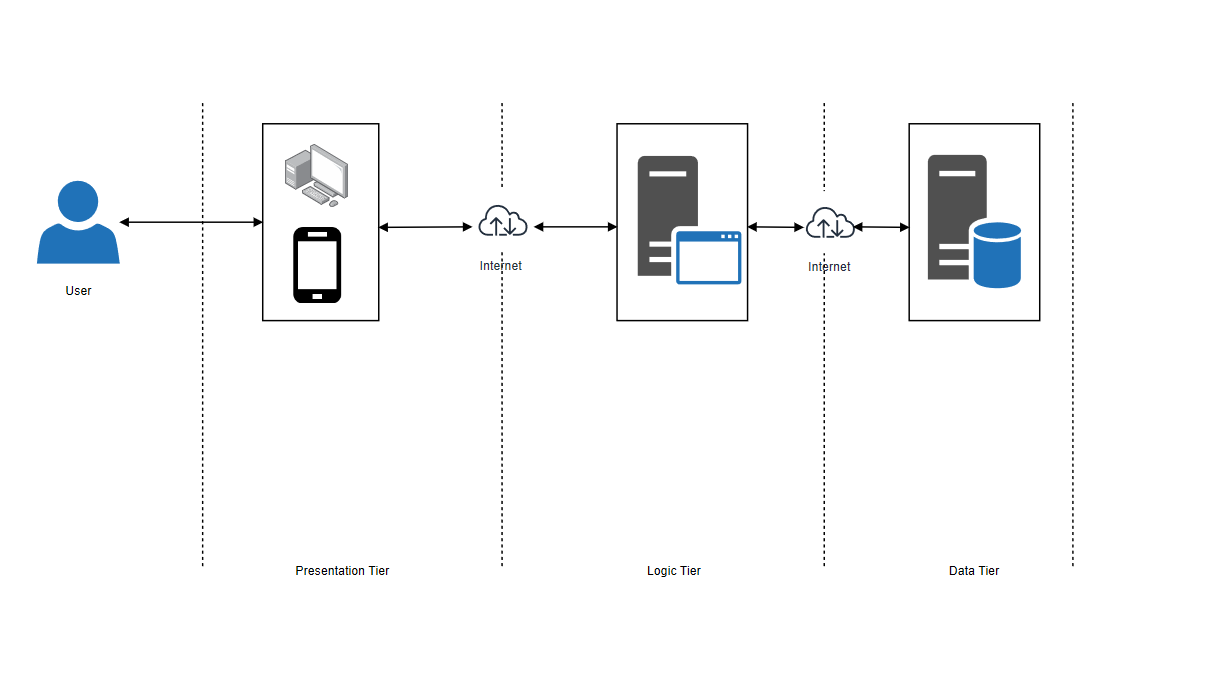
\includegraphics[width=\textwidth]{Images/three_layer}
	\caption{Three layer structure}
\end{figure}
\newline
As shown by the image above, the three layers consist in the presentation tier, the logic tier and the data tier
\begin{itemize}
\item Presentation Tier: consists of the user interfaces for all of the three clients (RegularUser, Policeman and MunicipalAuthority) and is used by the user to interact with both the application logic and Google Maps APIs \newline
\item Logic Tier: consists of the servers used to control the functionalities of the application, interacts with both the presentation and data tiers \newline
\item Data Tier: consists of the database server (where both user data and data generated by the application are stored), interacts only with the logic tier \newline
\end{itemize}
\newpage
\subsection{Component view}
\subsubsection{Introduction}
The following diagram represents the interface structure of the system, focusing on the application server structure. \newline
\begin{figure}[h!]
	\centering
	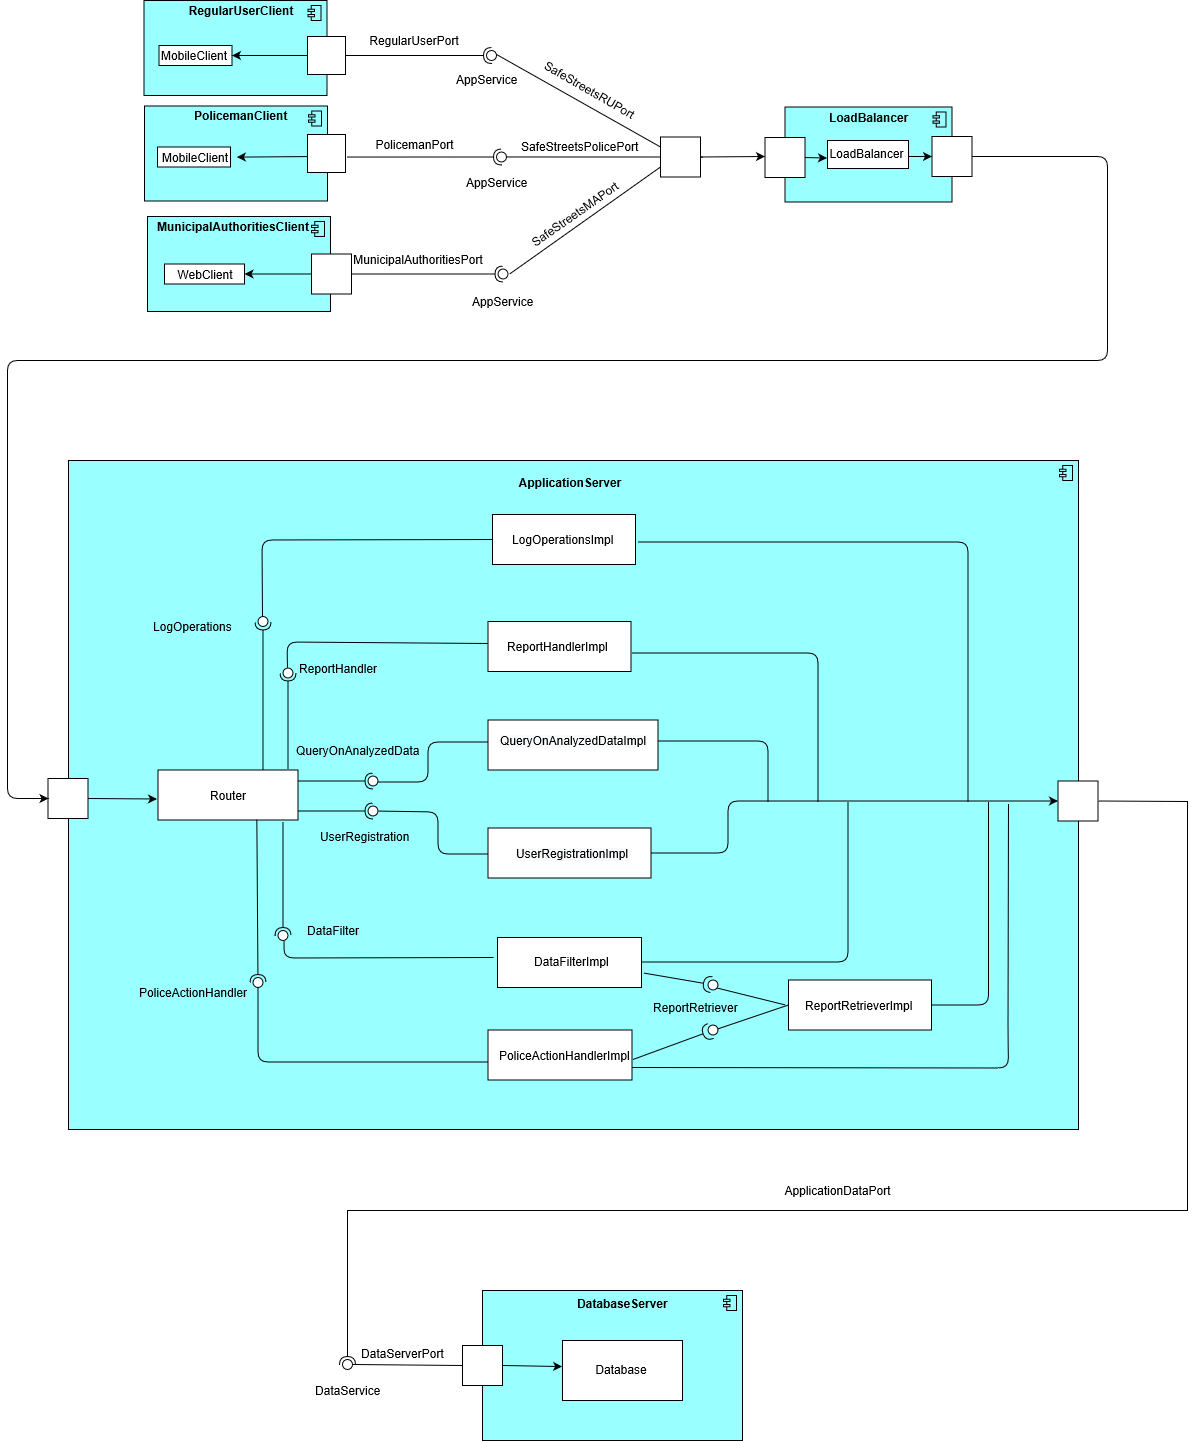
\includegraphics[width=\textwidth]{Images/component_diagram_beta}
	\caption{Component diagram}
\end{figure}

As shown above, the application logic is stored on the application server, while the clients just contain what is mandatory in order to contact the application server and to carry on basic operations  (thin client).\\
\subsubsection{Server}
We will now proceed to give a brief summary of the role of the components listed above:
\begin{itemize}
\item QueryOnAnalizedData: allows the RegularUser profiles to access data about the reports in a certain area or other information already analized by the MunicipalAuthorities
\item PoliceActionHandler: allows the policemen to take action on user made reports or to compile reports themself. The actions performed by the police consist in compiling reports (of which they will take care right away), marking themselves as dispatched towards a report, mark a report as wrong or signal that a traffic ticket has been written as a consequence of a reported traffic violation
\item ReportRetriever: this component is used by PoliceActionHandler and DataFilter in order to retrieve all the reports regarding the same violation (not just violation type, but also time, plate and location) as a given one. 
\item ReportHandler: this component manages users' submissions of reports about traffic violations. The reports are analyzed, authenticated and then strored inside the application DB
\item UserRegistration: this component allows the registration of all types of users. Note that, while RegularUser profiles registration is done by the user themselves, Authority profiles (Policeman and MunicipalAuthority) can only be registered by a system admin
\item LogOperations: this component takes care of the login and logout operations for all types of User profiles
\item DataFilter: allows MunicipalAuthority profiles to perform data-mining activities,  as well as cross-analyze external information (such as data about crashes in an area provided by a municipality ) with user-submitted reports
\end{itemize}
The logic of the application works based on the afromentioned components: they grant all the functionality needed to satisfy the system's goals (for a more in-depth analysis see chapter 4).
In the next two pictures more information about the system will be provided: the first represents a more accurate version of the class diagram presented in the RASD; the second includes a schema of the relationship between the classes interfaces and implementations of said interfaces. \newline
Please note that the "Device" class and the classes that extend it are not reported in the diagram, since they are not relevant to the purposes of this description. For any further information about these classes refer to the Class diagram in the RASD.

\begin{figure}[H]
	\centering
	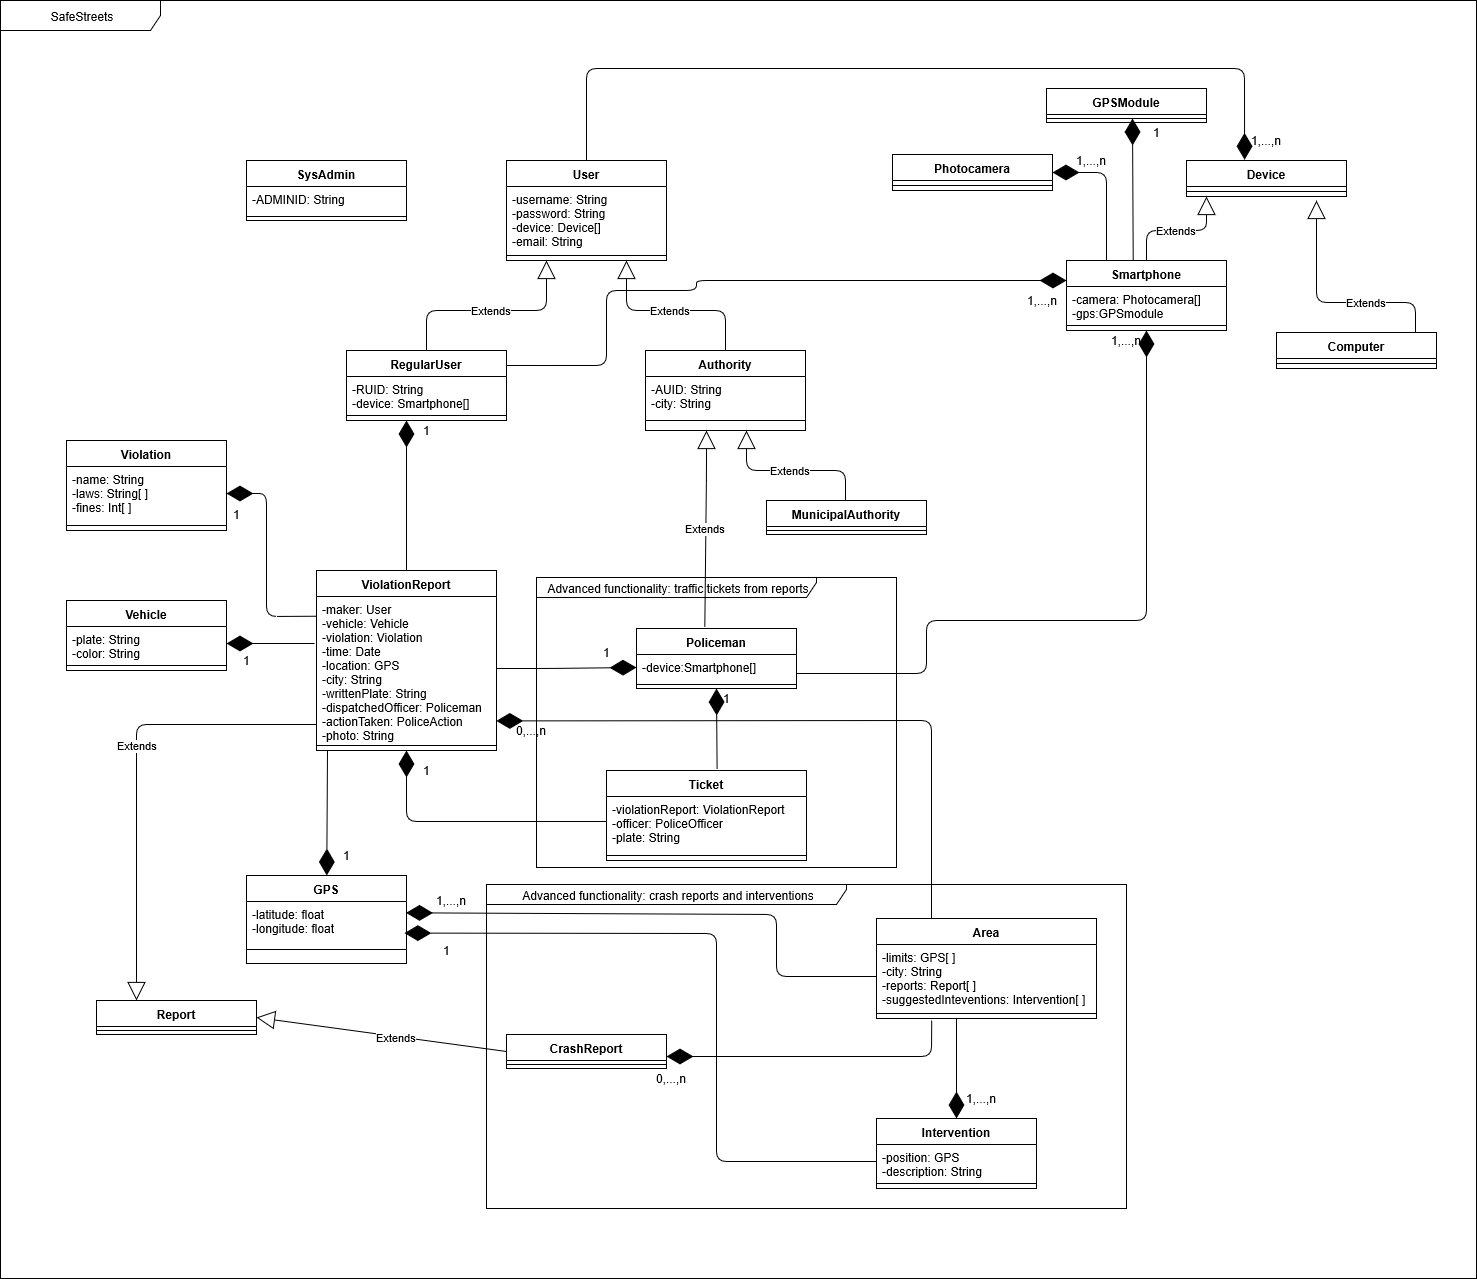
\includegraphics[angle=90, scale=0.35]{Images/ADV_class_diagram}
	\caption{Class diagram}
\end{figure}
\newpage

\begin{figure}[H]
	\centering
	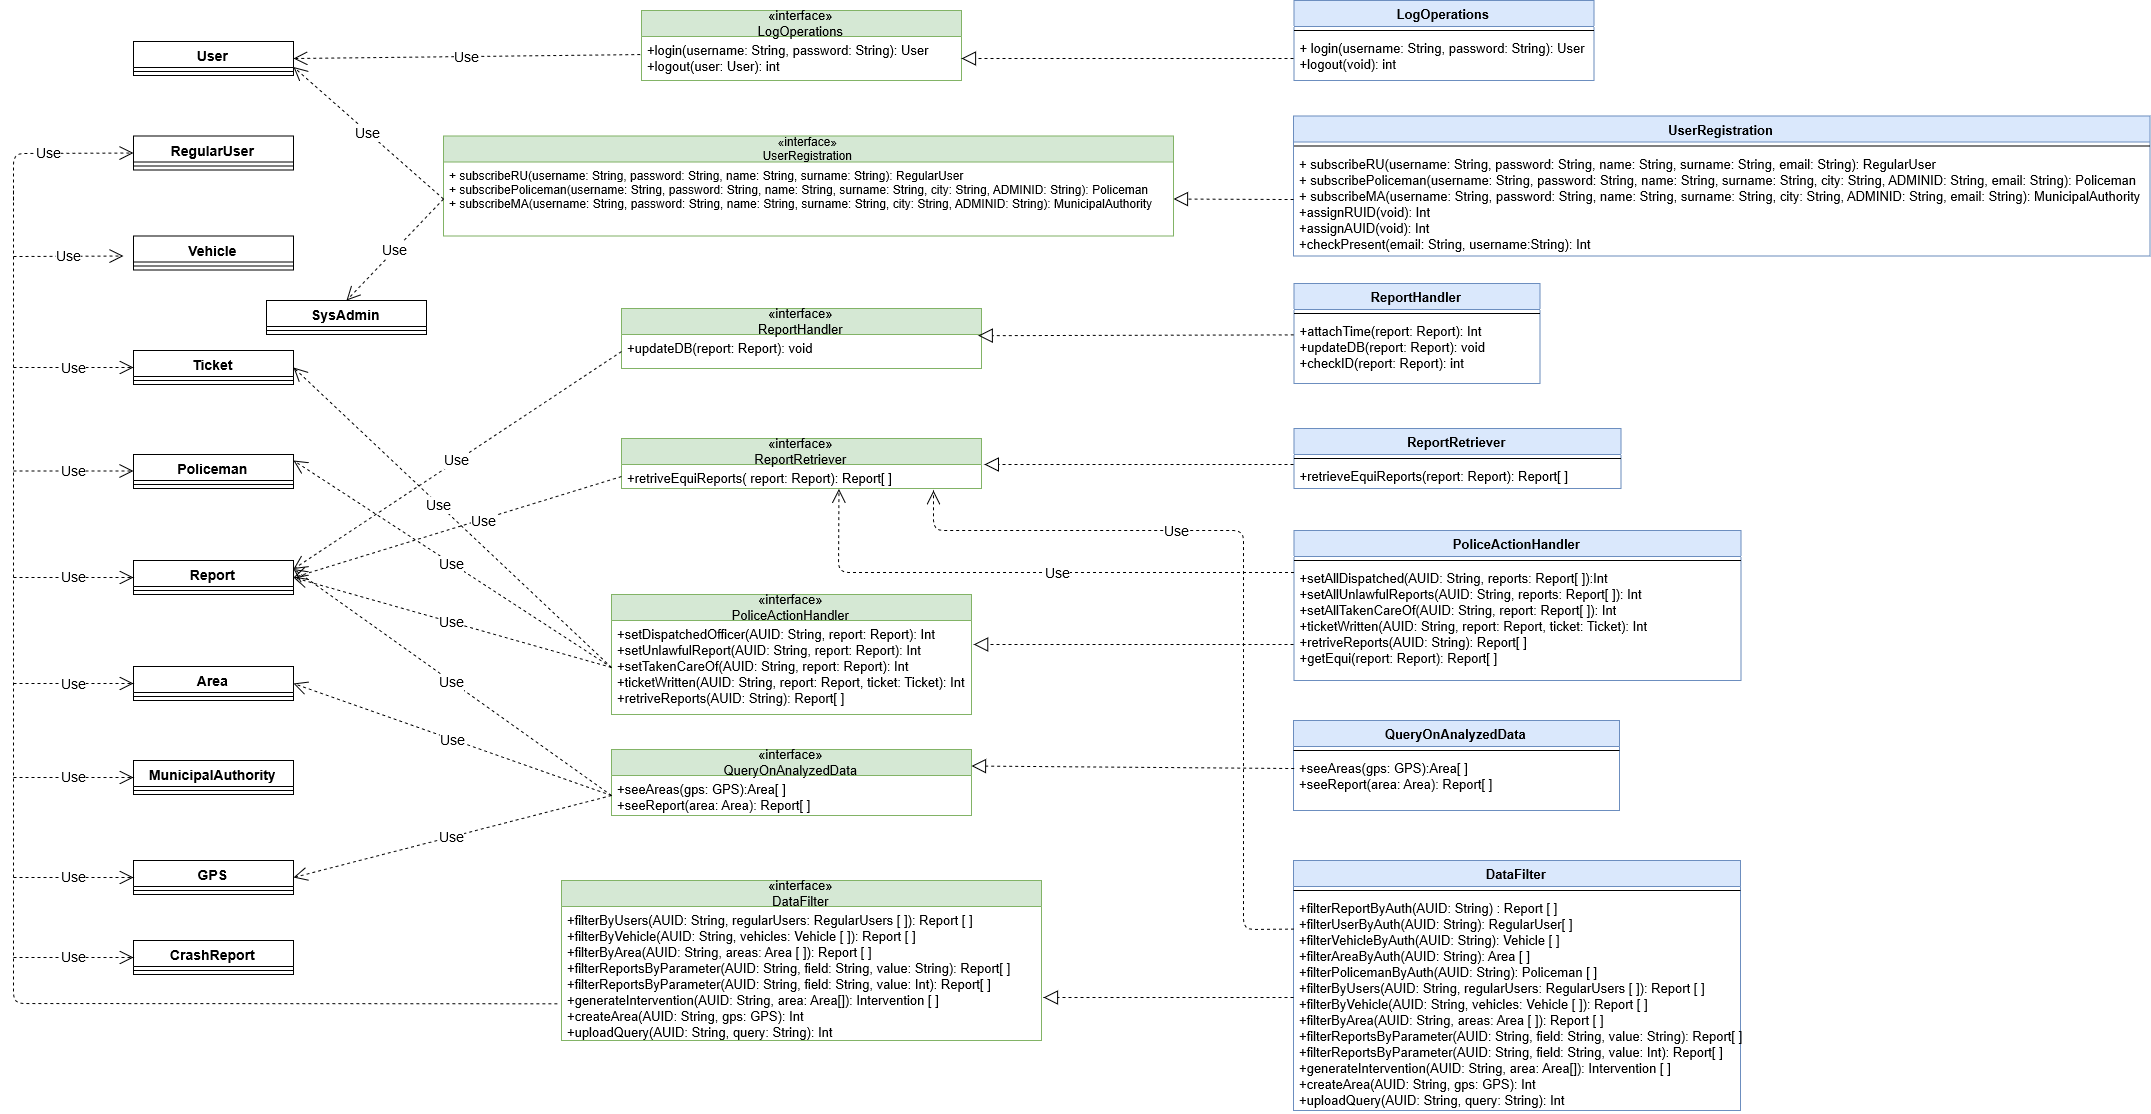
\includegraphics[angle=90, scale=0.25]{Images/component_class_relation}
	\caption{Relation between components and already specified classes}
\end{figure}
\newpage

\subsubsection{LoadBalancer}
The proprietary server approach chosen for the system may limit its scalability, since the available resources cannot be increased on the demand as in a cloud-based environment. Even though an high level of scalability is not a strict requirement for the application, we decided to insert a load balancer in order to achive better flexibility and scalability. This component should allow the system availability and funcionality even in case of heavy load, granting enough room to plan server expantions and simplifying these operations at the same time. \newline
A CISCO off-the-shelf solution is to be considered.

\subsubsection{Client}
In this section, we will give a description of the three clients functions showed in the introduction:
\begin{itemize}
	\item RegularUserClient: allows regular users to register and login to the service, to send reports about traffic violations and visualize on a map the most unsafe areas around him.
	\item PolicemenClient: allows policemen login to the service, to retrieve reports sent by the regular users (visualized in a map format) and to communicate that they are working to resolve a specific report.
	\item MunicipalAuthoritiesClient: allows municipal authorities to login to the service, to mine data about their municipality from the DataBase and to visualize violation maps, suggested interventions, advanced informations based on crossing SS data and accidents informations (if provided by the municipality).
\end{itemize}
In the following pictures we will provided more detailed informations about the three clients' components, focusing on one at a time.

\begin{figure}[h!]
	\centering
	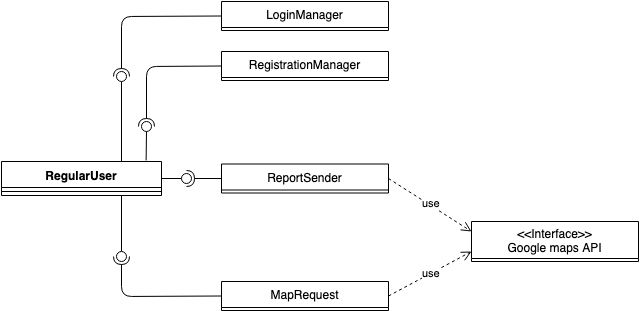
\includegraphics[scale=0.7]{Images/RegularUserClient}
	\caption{Relation between components inside regular user client}
\end{figure}
The components represented in this diagram are:
\begin{itemize}
	\item LoginManager: Allows users to send their log data to the server in order to login or logout from the system.
	\item RegistrationManager: Allows users to send  their registration data to the server in order to create a new account.
	\item ReportManager: Allows users to send a report about traffic violations, packing all the required data in a suitable format to be sent to the server. This component also uses Google maps API in order to recover informations about the area around user's geographical position.
	\item PlateRecognizer:
	\item MapViewer: Allows the user to visualize a geographical map from Google maps API enriched by data about unsafe areas, statistics and traffic violations coming from the server.
\end{itemize}

\begin{figure}[h!]
	\centering
	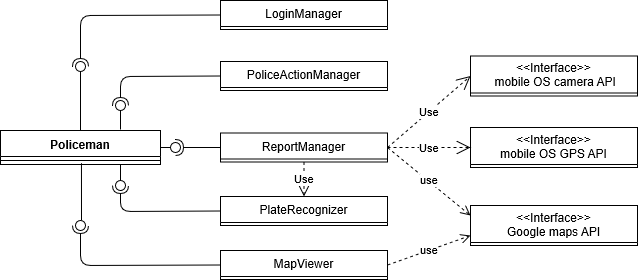
\includegraphics[scale=0.7]{Images/PolicemanClient}
	\caption{Relation between components inside policeman client}
\end{figure}

The components represented in this diagram are:
\begin{itemize}
	\item LoginManager: It has the same function as in the regular user client.
	\item ReportManager: Allows Policeman to send a traffic violation report with all the required data, packed in a correct format, to the server.
	This component also uses Google maps API in order to recover informations about the area around user's geographical position.\newline
	It's worth noting that if a policeman sends a report about a violation, he is automatically assigned to solving it.
	\item PlateRecognizer: 
	\item MapViewer: Allows a policeman to visualize the list of the various pending reportsfor his municipality.
	The locations of theeports will be shown on a map provided through Google maps API.
	\item PoliceActionManager: Allows a policeman to signal that his intention to take care of a report. This component will send a suitable message to server which will update its data accordingly, marking the considered report as under analisys.
	
\end{itemize}
\newpage
\begin{figure}[H]
	\centering
	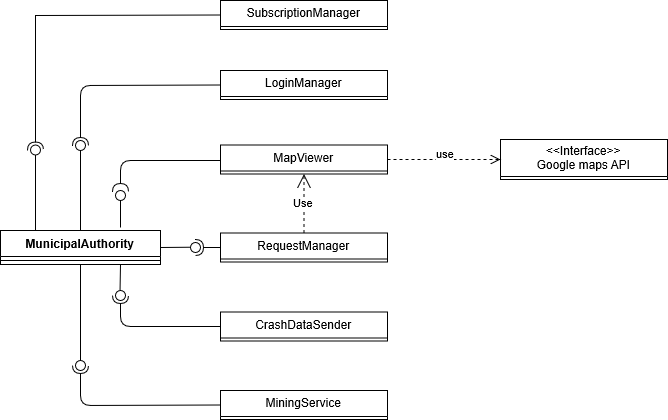
\includegraphics[scale=0.7]{Images/MunicipalAuthorityClient}
	\caption{Relation between components inside municipal authority client}
\end{figure}
The components represented in this diagram are:
\begin{itemize}
	\item LoginManager: It has the same function as in the regular user client.
	\item RequestManager: Allows the municipality to request data about Reports (solved or not) from the server. This componet uses MapViewer in order to provide violation data in a map format.
	\item MapViewer: Allows the visualization of the mined data in a map format. This component exploit Google Maps API to provide a representation of the local map.
	\item CrashDataSender: Allows the municipal authority to send Data about car crashes around the municipality to the server in order to be crossed with data already collected.
	\item MiningService: Provides an interface to simplify the acess of collected data to the municipality.
\end{itemize}

\newpage
\subsection{Deployment view}

\begin{figure}[h!]
	\centering
	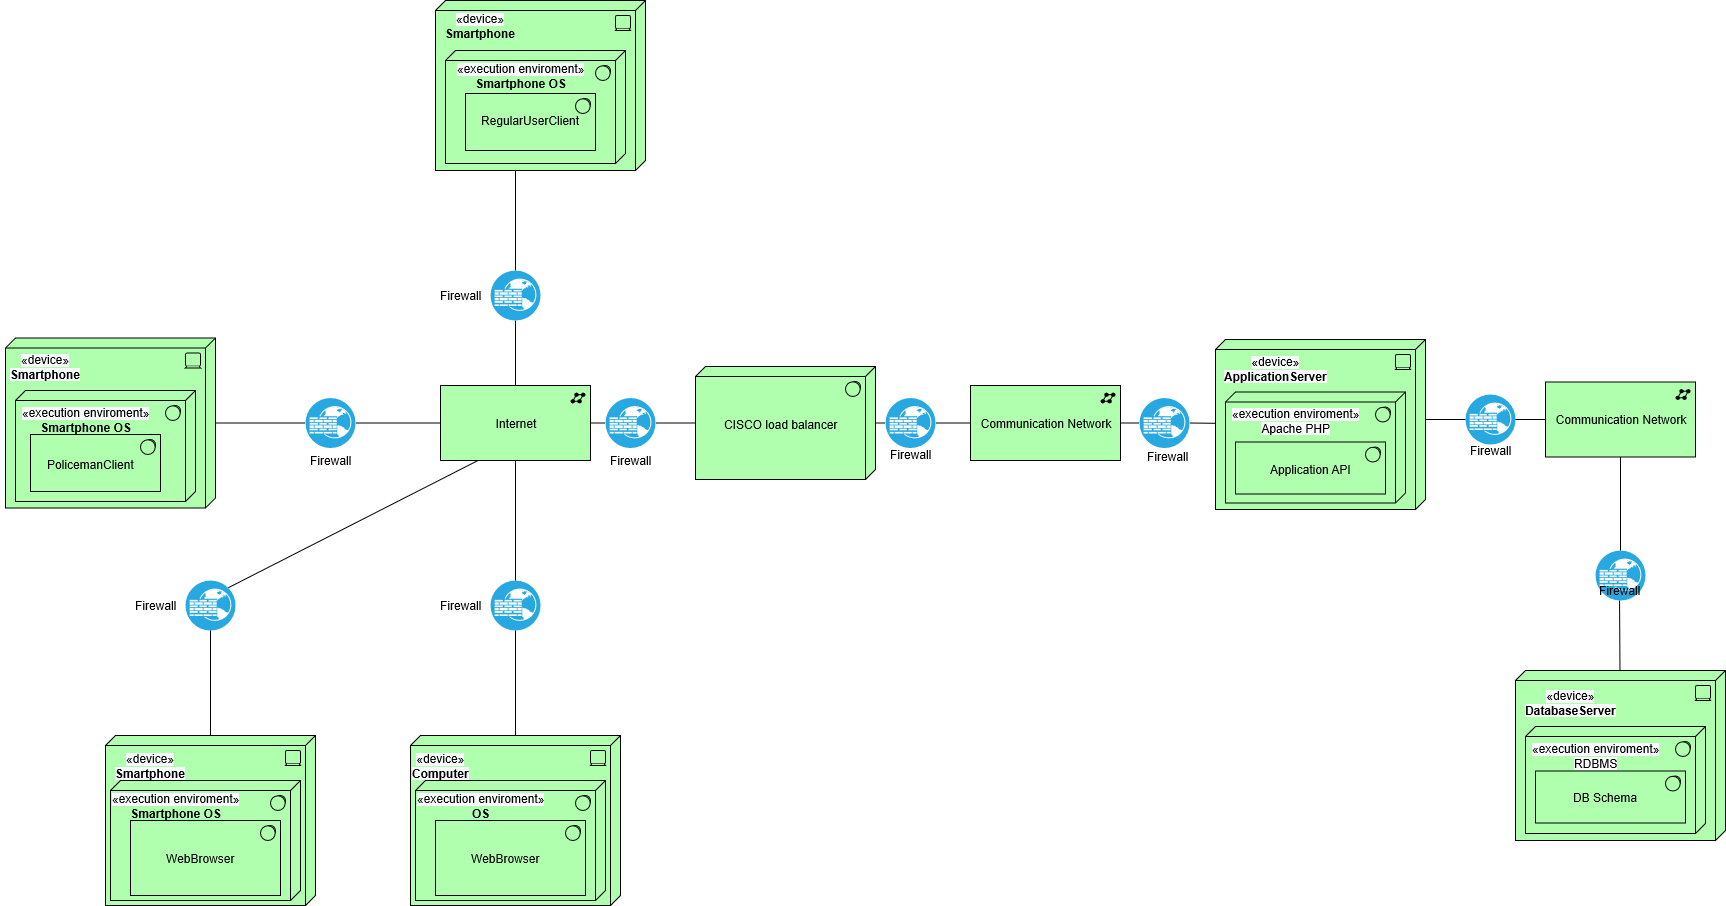
\includegraphics[width=\textwidth]{Images/physical_view}
	\caption{Physical view}
\end{figure}

The image above shows the system's architecture from a physical standpoint.
Components:
\begin{itemize}
\item Smartphone: Device used by both RegularUser and Policeman users type to interact with the application. Two different clients will be developed: one for regular users, that will allow them to look at already analyzed data and submit reports, and a different one for policemen, that will allow the officers make reports (upon which they will take actions right away) and take actions on reports
\item Computer: device used by MunicipalAuthorities users. They will interact with the application via a web page, that will allow them to interact in various ways with the Reports submitted by the other users.
\item Load Balancer: CISCO off-the-shelf load balancer
\item Application server: this server contains the application logic and will interact with the different clients in a client-server way.
\item DatabaseServer: this server contains the actual data, both about the registered users and related to the user submitted reports, the actions taken by the police and the results of the data mining operations done by municipal authorities
\end{itemize}
Please note that Google servers have not been included, since those servers will not be involved in the system deployment
\newpage

\subsection{Runtime view}
In this section the main functionalities of the system are analyzed through the use of sequence diagrams. The participants involved in the diagrams are either system componets (from client and server side) or external services APIs (e.g. Google Maps API) previuosly specified in this document.\newline
A colour schema has been used in order to increase diagram clarity: Client components are represented with light blue labels; Server components with yellow labels; third party API with green labels.

\medskip

\begin{figure}[H]
	\centering
	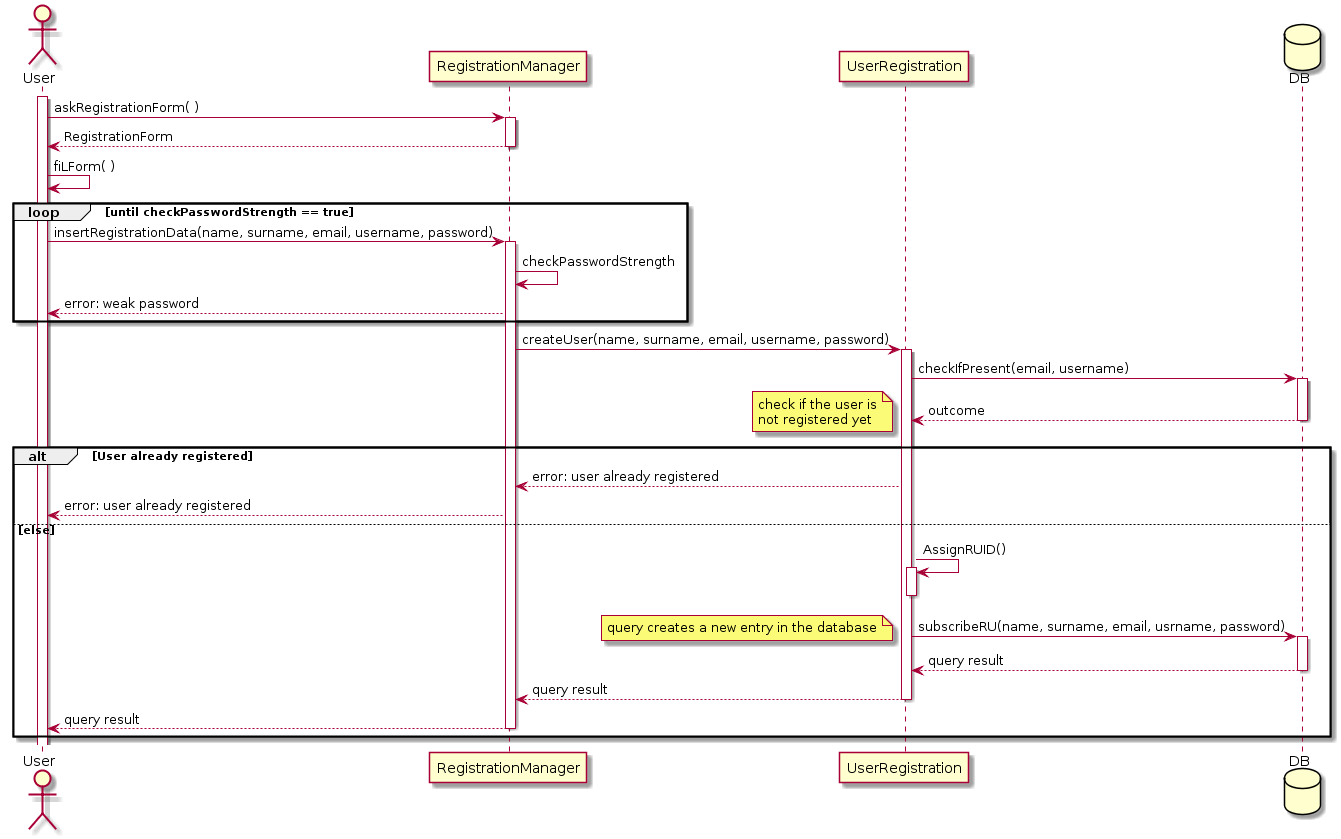
\includegraphics[width=\textwidth]{Images/seqDiag_userReg}
	\caption{User registration process}
\end{figure}
	\newpage

\begin{figure}[H]
	\centering
	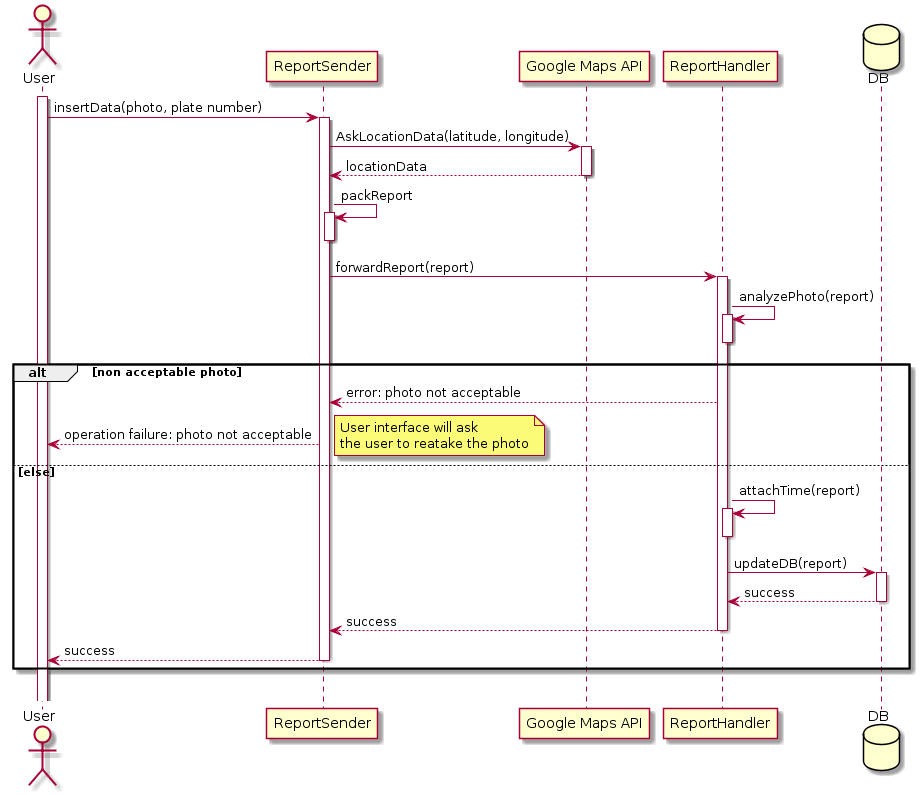
\includegraphics[width=\textwidth]{Images/seqDiag_ReportSignal}
	\caption{Report signaling procedure}
\end{figure}
	\newpage	
	
\begin{figure}[H]
	\centering
	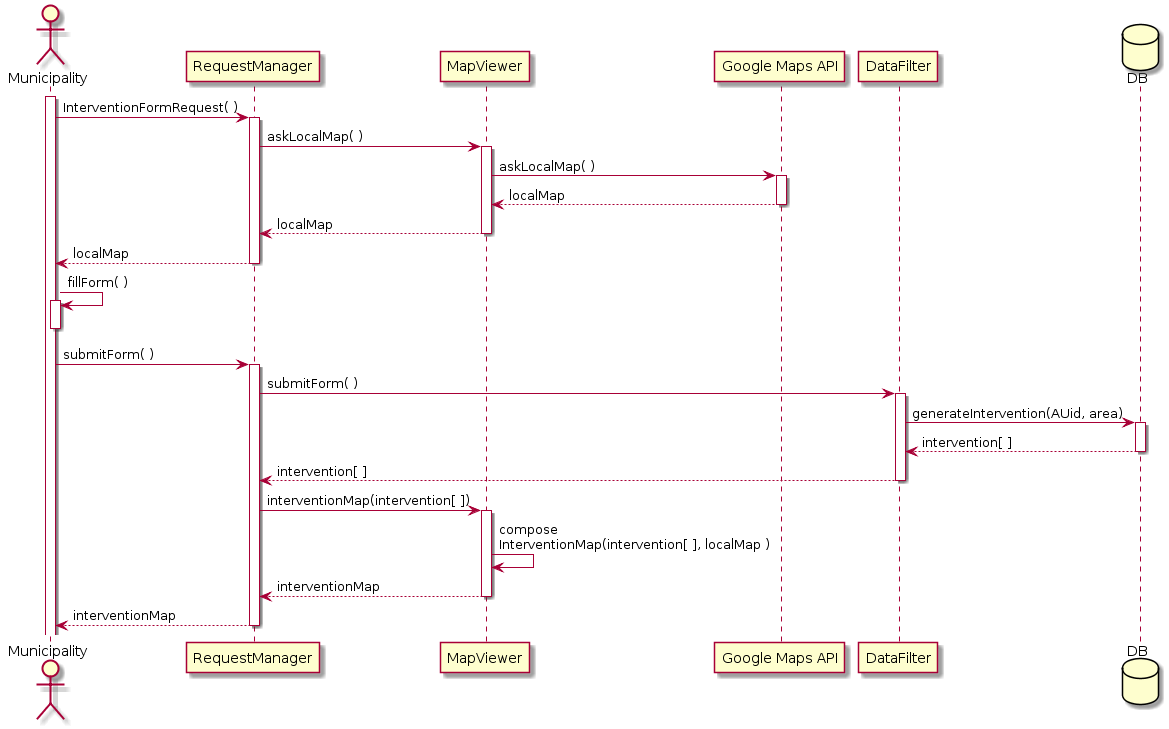
\includegraphics[width=\textwidth]{Images/seqDiag_Interventions}
	\caption{Municipality query for possible intervention in its metropolitan area}
\end{figure}
	\newpage

\begin{figure}[H]
	\centering
	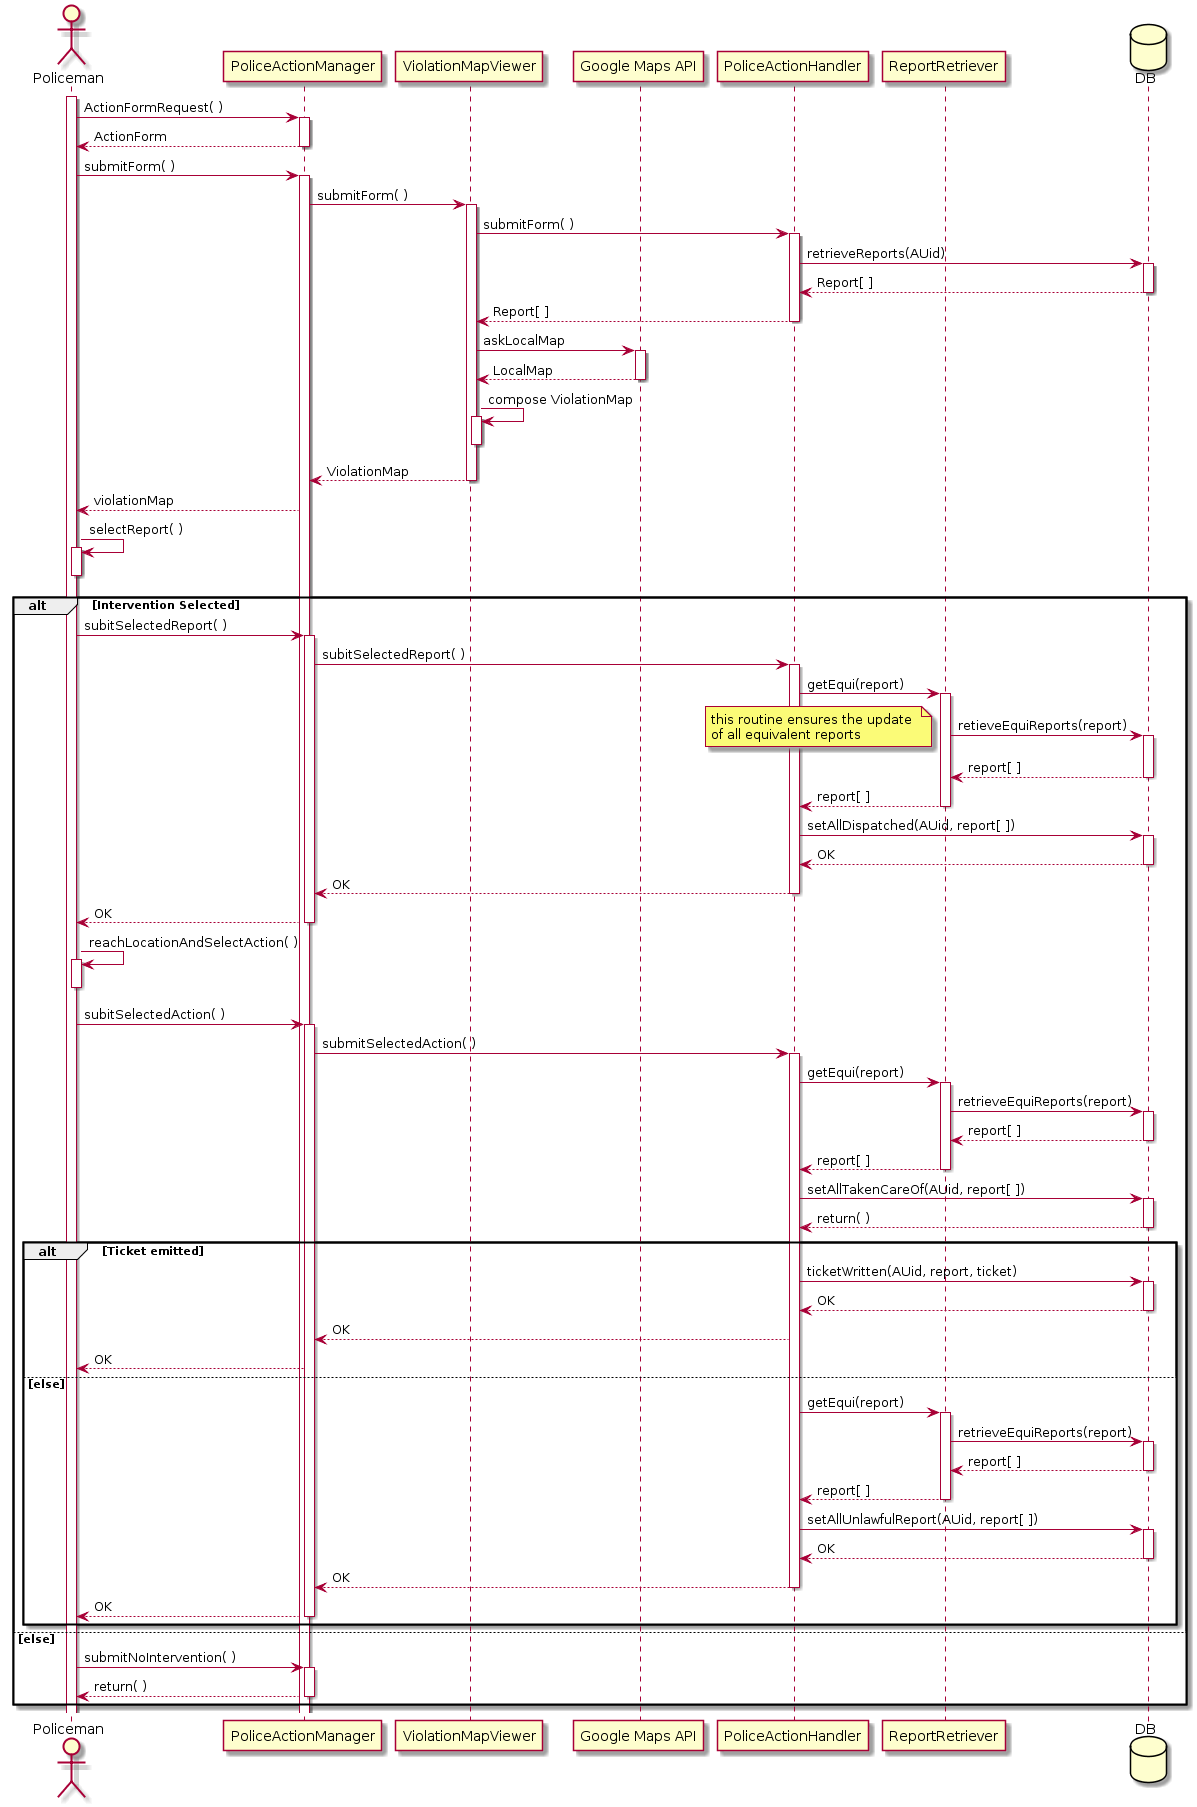
\includegraphics[width=\textwidth]{Images/seqDiag_PolicemanAct}
	\caption{Policeman takes care of a signaled report}
\end{figure}


\subsection{Interfaces}
\begin{figure}[H]
	\centering
	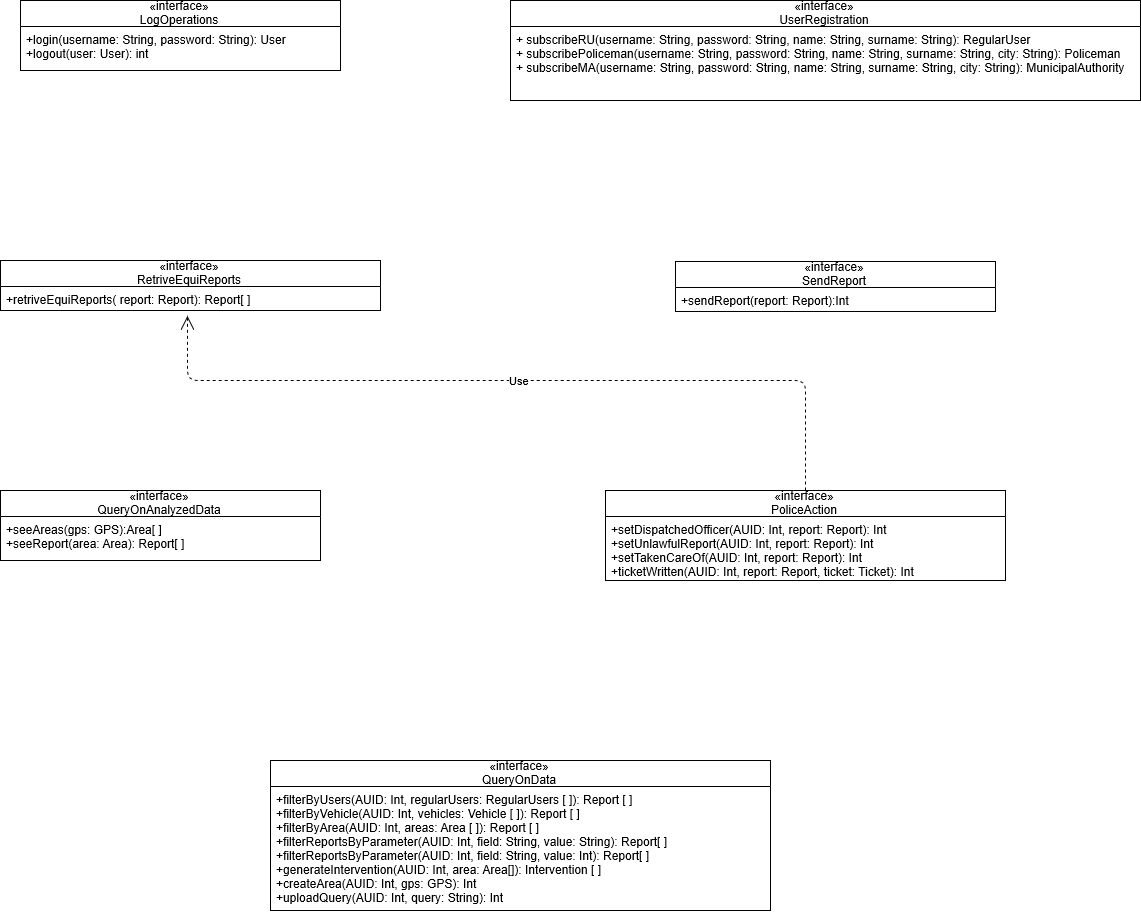
\includegraphics[width=\textwidth]{Images/interface_diagram}
	\caption{Components' interfaces}
\end{figure}
Other than the relation between PoliceActionHandler, DataFilter and ReportRetriever, already explained in section 2.2, it is worth noting that the interfaces don't actually expose all the methods of the objects that implement them. This choiche was made in order to hide the methods that will be called only from inside the object in which they are defined.
\newpage 

\subsection{Architectural and implementative styles and patterns}

\subsubsection{Architectural styles}
\begin{itemize}
	\item Client-server: given the nature of the application, a distibuted system in which data submitted by some users has to be accessible by other users, the figure of a mediator becomes necessary. Therefore a client-server architecture seems to be a good solution. Another alternative could have been a cloud computing architecture (SaaS, flex tenacity approach), but we opted for a client-server architecture since the workload and scalability issues would not be big enough to justify the increased costs.
	\item Thin client: in the aformentioned client-server architecture, the role of the server is more than just a message manager. As a matter of fact, the server also takes care of the application logic, allowing a light client with limited functionalities.
	\item Three tiers architecture: given the client-server with thin client architecture described, the most natural solution is a three tier architecture in which the presentation layer is on the client, the application layer on the application server and the data layer on the database server. 
\end{itemize}

\subsubsection{Design patterns}
\begin{itemize}
	\item Model-view-controller: given the three-tiers and thin client architecture, using a MVC design pattern is quite easy: the model will be represented by the database server, the control by the application server and the view will be managed by the client. \newline
	The development of a different view for each type of user will be necessary, considering the different privileges and functions offered. Thus, in this section of the system modularity of the application will be central: sharing of common modules will simplify the development. 
	\item Facade: used to hide the application server's components complexity
	\item Factory: used in RegularUser and Policeman clients to create reports
\end{itemize}

\subsection{Other design choiches}
\begin{itemize}
	\item Security concerns: as expressed in the RASD, there are various measures needed in order to obtain a good level of security:
	\begin{itemize}
		\item Fileting and escaping registartion requests of all kinds of user profiles and RegularUser submitted reports (Policeman submitted ones and MunicipalAuthority queries are considered trustwothy) in order to avoid code injections
		\item Escaping and filetring login fields in order to avoid code injections
		\item All communication must happen over a secure channel (HTTPS)
		\item An anti cross site request forgery token is needed 
	\end{itemize}
	\item Database: for this application a relational database has been chosen, since involving any other kind of solution would be a waste of resources for no sensible inprovement on the system
	\item All exchanged data are in xml format (all the photos are hahsed via base 64 and embedded in the document)
\end{itemize}

%------------------------------------------------------------------------------------------------------------------------------------------------
\clearpage
{\color{Blue}{\section{User Interface}}}
\label{sect:UI}
Interfaces mock-ups have already been presented in the RASD documentation.
They can be found in the section 3.1.1 of the RASD. \par
It's remarkable that, since regular users and policemen clients interfaces share a lot of functions, it is recommended a modular approach in order to simplify the development.

%------------------------------------------------------------------------------------------------------------------------------------------------
\clearpage
{\color{Blue}{\section{Requirements traceability}}}
\label{sect:requirements}
\subsection{External interface requirements}
 
	\subsubsection{User Intefaces}
	\begin{figure}[h!]
		\centering
		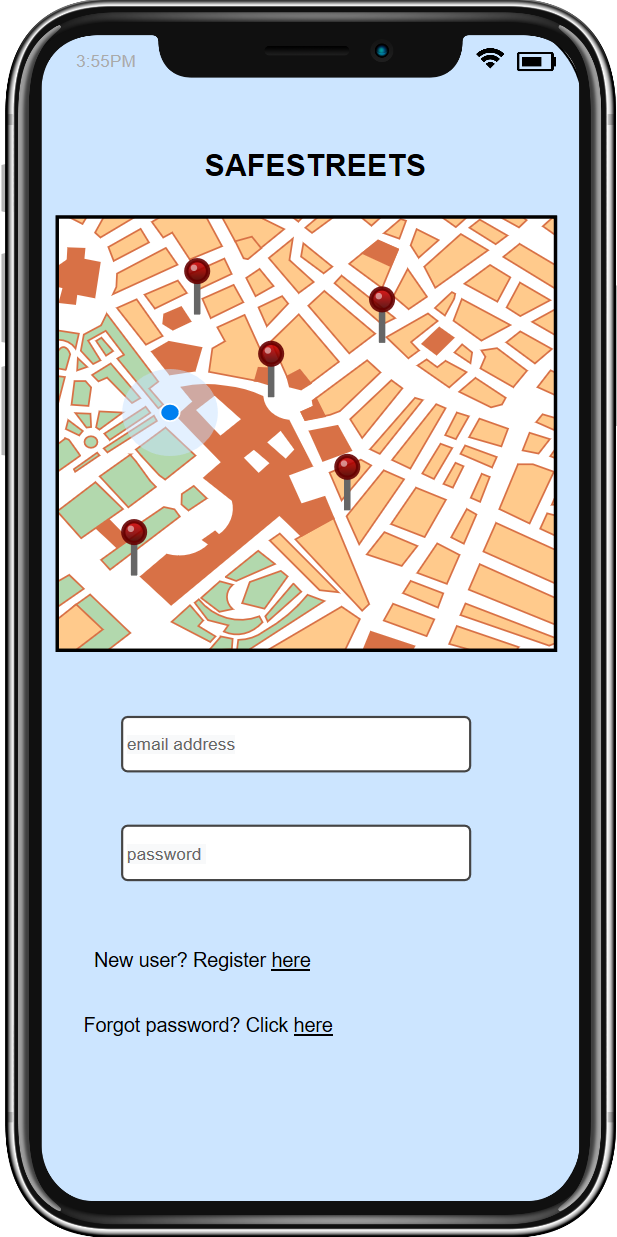
\includegraphics[scale=0.55]{Images/login_mockup}
		\caption{Mockup of the login page}
	\end{figure}
	\newpage
	\begin{figure}[h!]
		\centering
		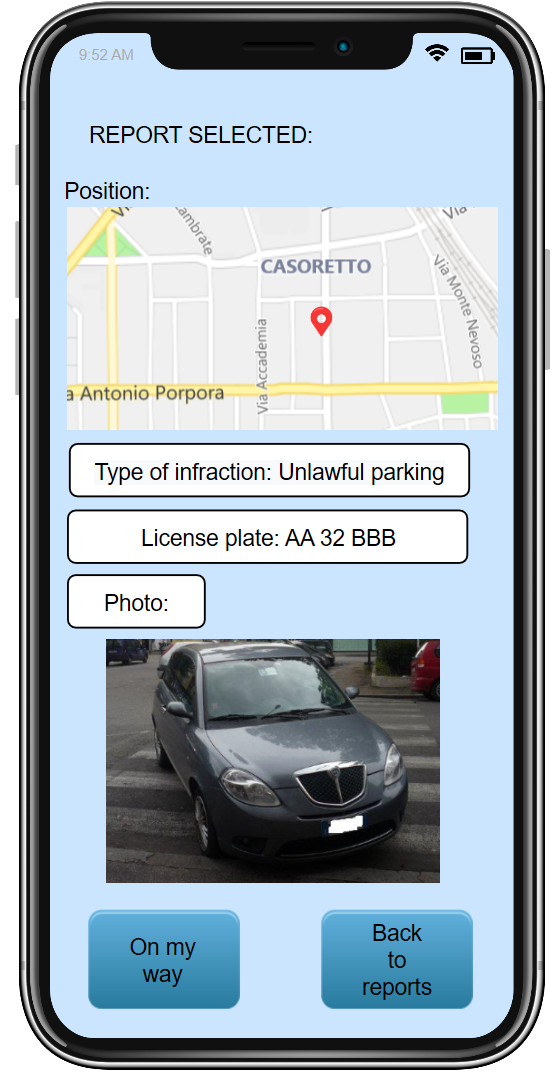
\includegraphics[scale=0.65]{Images/Policeman_client_mockup}
		\caption{Mockup of part of the police client}
	\end{figure}
    \newpage
    \begin{figure}[h!]
    	\centering
    	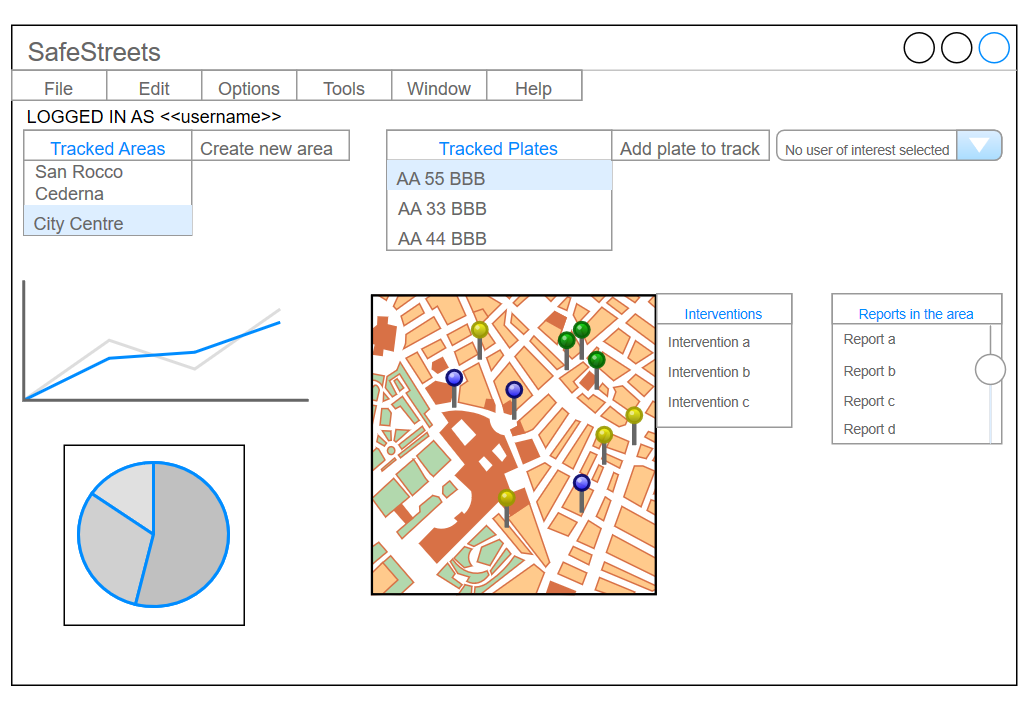
\includegraphics[angle=90, scale=0.55]{Images/MunicipalAuthority_client_Mockup}
    	\caption{Mockup of the municipal authority client}
    \end{figure}
	\subsubsection{Hardware Interface}
	\subsubsection{Software Interfaces}
	\subsubsection{Comunication Interface}
	
\subsection{Functional Requirements}
\bigskip

\begin{enumerate} [label = G\arabic* - ]

\item \textbf{Allow users to signal traffic violations}
	\begin{itemize}
	\item (R1) SS user client must provide a registration interface.
	\item (R2) SS must assign a unique ID to each registered user.
	\item (R3) SS user client must provide a violation report function.
	\item (R4) SS should verify each report is sent from an existent ID.
	\end{itemize}
	\bigskip
	
\item \textbf{Allow users to include pictures in violation reports}
	\begin{itemize}
	\item (R5) Application must have permission and access to the device camera.
	\item (R6) Pictures should be taken through camera inside the application to ensure protection against manipulations.
	\end{itemize}
	\bigskip
	
\item \textbf{The system must be able to retrieve the geographical position of a violation and add it to the report}
	\begin{itemize}
	\item (R7) Application must have permission and ability to access to GPS service offered by the smartphone device.
	\end{itemize}
	\bigskip
	
\item \textbf{The system must recognise (from pictures) license plates}
	\begin{itemize}
	\item (R8) The system should implement an image recognition algorithm.
	\item (R9) The system should ask the user to manually insert the license plate number of the offender car pictured in the provided photo for data integrity purposes.
	\end{itemize}
	\bigskip

\item \textbf{The system must store user made reports}
	\begin{itemize}
	\item (R10) SS must have a consistent database.
	\item (R11) Every report received has to be saved in SS database.
	\item (R12) SS must ensure that data cannot be tampered with.
	\end{itemize}
	\bigskip
	
\item \textbf{Allow users and authorities to mine information collected by the application}
	\begin{itemize}
	\item (R13) SS should provide an authoriteies dedicated client.
	\item (R14) SS authority client should provide a registration function.
	\item (R15) SS should provide the APIs and the tools to allow mining information by 3rd party.
	\item (R16) SS should implement an automated tool for data analysis and display.
	\end{itemize}
	\bigskip
	\end{enumerate}
	
\begin{enumerate} [label = GA 1.\arabic* - ]

\item \textbf{The system must be able to cross the data collected with information about the accidents coming from the municipality} 
	\begin{itemize}
	\item (R17) The involved municipality should provide incidents data of his metropolitan area.
	\item (R18) Data access interfaces should be provided by municipality or defined by SS designers in collaboration with people from the municipality.
	\item (R19) The system should have already collected a suitable amount of data.
	\end{itemize}
	\bigskip
	
\item\textbf{The system must be able to suggest possible interventions to decrease the risk of violations in unsafe areas}
	\begin{itemize}
	\item (R16) SS should implement an automated tool for data analysis and display.
	\end{itemize}
	\bigskip
\end{enumerate}

\begin{enumerate} [label = GA 2.\arabic* - ]
	
\item \textbf{Allow the local police to retrieve data about violation to generate traffic tickets}
	\begin{itemize}
	\item (R20) SS should provide a dedicated client to police officers.
	\end{itemize}
	\bigskip
	
\item \textbf{The system must be able to ensure the veracity of the information sent by the users}
	\begin{itemize}
	\item (R2) SS must assign a unique ID to each registered user.
	\item (R3) SS should verify each report is sent from an existent ID.
	\item (R21) SS should include anti-flooding protection mechanism (e.g. timer for each ID).
	\item (R6) Pictures should be taken through camera inside the application to ensure protection against manipulations.
	\item (R22) Report forward to DB should exploit a secure and encrypted channel.
	\end{itemize}
	\bigskip

\item \textbf{The system must track whether the police has taken care of a certain violation}
	\begin{itemize}
	\item(R23) SS policeman client should offer a function to signal that a traffic ticket (related to a previous) has been generated.
	\item(R24) SS stores in its DB traffic ticket emission alongside the corresponding report.
	\end{itemize}
	\bigskip
	
\item \textbf{Traffic tickets must be issued to the person that owns the vehicle that committed the violation}
	\begin{itemize}
	\item(R25) The system must ensure that the traffic ticket emission signalling (policemen client) is available only for taken care reports.
	\item(R26) SS will ask the officer the license plate number and will accept to signal ticket emission only if the inserted number match the one contained in the report.
	\end{itemize}
	\bigskip
	
\item \textbf{The system must be able to build statistics from the information about issued tickets}
	\begin{itemize}
	\item(R16) SS should implement an automated tool for data analysis and display.
	\end{itemize}
	\bigskip
	
	\end{enumerate}

	\subsubsection{Scenarios}
	\begin{enumerate}
	\item \textbf{Bad Parking}: Bob is a commuter and every morning needs to reach the train station by car: the daily struggle to park his car in the surroundings is even worsened by parking violations. One morning, coming across another car occupying two parking slots, Bob decides to start contributing to SafeStreet service and its violation map: he downloads and installs SS app, accepts to grant Camera and GPS authorizations to it and fills a brief form for the registration. Once logged in, he uses the dedicated report feature. He takes a picture of the violation, inserts manually the license plate number and, after the application completes the verification of the inserted data, he sends the violation report, which also includes the GPS location and the current time.
 	\item \textbf{An anxious mother}: every day Laura lets his 12 years old son walk to school by himself. One day she hears about SS, a new app providing information about traffic violation in her city, and thinks that it can be useful to check if her son daily walking route is reasonably safe or not. Using SS violation map, which provides a street level highlight of violation distribution, she finds out that his son usually walks in potentially unsafe streets, with cars parked on sidewalks forcing pedestrians to walk in the middle of the street, and suggests him a new route based on the map provided by SS.
	\item \textbf{Smart Municipality}: Milan municipality is looking for a large data set regarding traffic monitoring for his metropolitan area. The administration aims to mine useful information from it in order to identify critical areas and plan interventions. They found out SS and its violation DB, so they subscribe to the service as a public institution filling a required form and gain access to the needed data. With high privilege data access granted to public authorities, SS provide them a suitable amount of data for the administration goal.
	\item \textbf{Traffic Monitoring Service}: Gotham City municipality has just introduced a new traffic plan in one of his main districts and wishes to track in an accurate way the evolution of traffic violations. SS should do the trick: Gotham municipality registers to SS service as public authority and now can have privileged access to the data collected by the application. However, Gotham City has no infrastructure dedicated to large data set mining. No worries: the impact of the new traffic plan can be evaluated exploiting built-in SS violation map and traffic tickets emission trends.
	\item \textbf{SafeStreet for Safer Cities}: the city of Monza provide a dedicated service offering data about incidents on its territory. SS has exploited its advanced features to cross its own information about traffic in Monza with the data provided, identifying possible unsafe areas and suggesting possible interventions. The administration of the city knows that managing the traffic plan of a vast city is complex and find that SS automated analysis could really lower effort and costs of the operations. Thus, the municipality decides to register to SS services and to exploit its traffic monitoring and intervention suggestion tool. 
	\item \textbf{Traffic Tickets}: NotSoSafe City is struggling trying to guarantee a decent level of violation control in his vast metropolitan area, considering his personnel available is limited. The municipality come to know that SS provide an efficient violation signalling service and a dedicated police officer client that even tracks ticket emissions. After registration as a public institution, the municipality issue to every policeman the installation of SS client on corporate (or personal) phone. Policemen can now take advantage of the real-time violation notification service of SS app for quick interventions if needed. Moreover, SS violation map offers the municipality a strong tool to simplify territory control: officer patrol activity can be directed to the most unsafe areas reported by the application.
	\item  \textbf{Policeman Intervention}: Anna is a police officer working for Rome municipality. The city administration has recently decide to exploit SS service in order to optimize traffic ticket emission. Anna is patrolling district one and suddenly receive a violation notification from SS client installed on her smartphone. The report is coming from a nearby street so Anna decide to take care of the report, marking that an officer has been dispatched  through the dedicated app function. Once on place, Anna verifies that the violation reported has truly occurred and issues a traffic ticket. She finally marks the report as” taken care” within SS app and gets back to her patrolling activity.
	\end{enumerate}
	
	
	\subsubsection{Use Case Description}
	\medskip
	
	\begin{enumerate}
	\item \textbf{User Registration}
		\begin{table}[h!]
		\begin{tabular}{|l|p{12,5cm}|}
		\hline
		Actors            			&       	User\\ \hline
		Goals             			&         G1\\ \hline
		Entry Conditions  	&  		User opens the mobile app for the first time\\ \hline
		Event Flow        		&          
				\begin{enumerate}[label=\alph*)]
					\item The user accepts to grant SS permission to access camera and GPS.
					\item SS user interface shows a menu with Log In and Sign Up options.
					\item The user taps on Sign Up opening the registration form.
					\item The user fills at least the mandatory fields with required personal information.
					\item The user accepts SS privacy policy by ticking a box.
					\item The user confirms the registration by cliking on a link sent to the inserted e-mail account.
				\end{enumerate}\\ \hline
		Output Conditions &    		The user completes the registration and can access SS features.	\\ \hline
		Exceptions        		&       	
				\begin{enumerate}[label=\alph*)]
					\item The user does not accept required permissions. In this case the app will close.
					\item The user is already registered. An error message is displayed asking to reinsert the data is displayed.
					\item Mandatory fields are left empty or filled with invalid entries. An error message is displayed asking to reinsert the data is displayed.
					\item The user does not accept privacy policy. An error message is displayed asking to accept the policy is displayed.
					\item Verification link expires before user confirms registration. In this case the account is deleted from SS system.
				\end{enumerate}\\ \hline
	\end{tabular}
	\end{table}
	
	\clearpage
	
	\item \textbf{Institution Registration}
		\begin{table}[h!]
		\begin{tabular}{|l|p{12,5cm}|}
		\hline
		Actors            			&       	Institution/Authority\\ \hline
		Goals             			&         	G6, GA2.1\\ \hline
		Entry Conditions  	&  		No entry condition\\ \hline
		Event Flow        		&          
				\begin{enumerate}[label=\alph*)]
					\item The institution connects to SS website.
					\item In the website institution dedicated area, the authority finds a mandatory registration form. A certificate for institution acknowledgement must be provided as part of the form.
					\item The institution fills all the mandatory fields and accepts privacy policy.
					\end{enumerate}\\ \hline
		Output Conditions &    		Registration successfull: the institution can access advanced SS features.\\ \hline
		Exceptions        		&
				\begin{enumerate}[label=\alph*)]
					\item The institution is already registered.
					\item Mandatory fileds are incomplete.
					\item Certificate is missing.
					\item The institution does not accept Privacy policy.
				\end{enumerate}
				All exceptions raise an error asking to complete the unfulfilled operations. \\ \hline
	\end{tabular}
	\end{table}
	
	\item \textbf{Violation Signaling}
		\begin{table}[h!]
		\begin{tabular}{|l|p{12,5cm}|}
		\hline
		Actors            			&       	User\\ \hline
		Goals             			&         G1, G2, G3, G4, G5	\\ \hline
		Entry Conditions  	&  		User is registered, logged in the mobile app and wants to signal a violation\\ \hline
		Event Flow        		&          
				\begin{enumerate}[label=\alph*)]
					\item The user opens SS app and taps on the "Signal a Violation" option.
					\item The user selects one of the possible violations presented in graphic menu.
					\item The app asks the user to attach a photo of the violation, picturing the vehicle involved with license plate visible, and to manually insert license plate number of the vehicle.
					\item The user takes a photo of the violation within SS app and insert license plate number of the vehicle.
					\item The app localy verifies if the license plate pictured and the manually inserted one match and readies the violation report. 
					\item The app shows a menu displaying a " Send Report" and a "Cancell" options.
					\item The user tap on "Send Report" in order to send the violation report to SS systems.
					\end{enumerate}\\ \hline
		Output Conditions &    		The report is sent to SS server and it is stored in a suitable database.\\ \hline
		Exceptions        		&       	
				\begin{enumerate}[label=\alph*)]
					\item License plate number recognized by the app and the one manually inserted do not match. In this case, an error message is raised and SS asks the user to retake the photo.
				\end{enumerate}\\ \hline
	\end{tabular}
	\end{table}
	
	\item \textbf{Providing Useful Information to Users}
		\begin{table}[h!]
		\begin{tabular}{|l|p{12,5cm}|}
		\hline
		Actors            			&       	User\\ \hline
		Goals             			&         G6, GA2.5\\ \hline
		Entry Conditions  	&  		User is registered, logged in the mobile app and wants to consult violation information\\ \hline
		Event Flow        		&          
				\begin{enumerate}[label=\alph*)]
					\item The user opens SS app and taps on the "Statistics" option.
					\item The user selects the prefered function in the menu displayed (e.g. violations maps, traffic tickets statistics). \newline
								Note: functions availability may vary depending on the service offered by the city municipality.
				\end{enumerate}\\ \hline
		Output Conditions &    		The user acess to the requested service.\\ \hline		
				
		Exceptions        		&       	
				\begin{enumerate}[label=\alph*)]
					\item The user requests a service not available in his city. An error message explaining the reasons of the function absence is displayed.
				\end{enumerate}\\ \hline
	\end{tabular}
	\end{table}
	
	\item \textbf{Providing Data to Mine to Istitutions}
		\begin{table}[h!]
		\begin{tabular}{|l|p{12,5cm}|}
		\hline
		Actors            			&       	Institution/authority\\ \hline
		Goals             			&         	G6\\ \hline
		Entry Conditions  	&  		Institution is registered to SS service and desires to access to data it collects\\ \hline
		Event Flow        		&          
				\begin{enumerate}[label=\alph*)]
					\item The institution specifies a proper query for the data required.
					\item The system verifies if the query author is an registered acknowledge.
					\end{enumerate}\\ \hline
		Output Conditions &    		Requested data is provided to the institution. \\ \hline
		Exceptions        		&
		       	\begin{enumerate}[label=\alph*)]
		       		\item The query is not well formatted. An error is reported and the transaction is aborted.
		       		\item The query author is not recognized. An error is reported and the request is not fullfilled. 
		       	\end{enumerate}\\ \hline
	\end{tabular}
	\end{table}
	
		\clearpage
	
	\item \textbf{Providing Institution Intervention Suggestions}
		\begin{table}[h!]
		\begin{tabular}{|l|p{12,5cm}|}
		\hline
		Actors            			&       	Institution/Authority\\ \hline
		Goals             			&         	GA1.2\\ \hline
		Entry Conditions  	&  		Institution is registetred to SS service and desires to access to "Suggested Intervention" advanced feature\\ \hline
		Event Flow        		&          
				\begin{enumerate}[label=\alph*)]
					\item The institution logs in the SS website
					\item The institution navigates to the "Suggested Intervention" sections
					\item In the interface displayed the institution searches the areas of interest for possible intervention suggestions
					\end{enumerate}\\ \hline
		Output Conditions &    		The institution can access to intervention suggestions for the selected area\\ \hline
		Exceptions        		&       	
				\begin{enumerate}[label=\alph*)]
					\item The institution fails to login in the website page. An error message asking to reinsert credential is displayed.
					\item In the selected area there are no suggested intervention. An error message explaining the absense of possible intervention is reported.
				\end{enumerate}\\ \hline
	\end{tabular}
	\end{table}
	
	\item \textbf{Police Officer Takes Care of a Report}
		\begin{table}[h!]
		\begin{tabular}{|l|p{12,5cm}|}
		\hline
		Actors            			&       	Police Officer\\ \hline
		Goals             			&         	GA2.1, GA2.3\\ \hline
		Entry Conditions  	&  		The police officer receives a notification on her/his SS mobile client and decides to take action\newline
													\centerline{OR}\newline
													The police officers finds in the SS client dedicated section an available violation report and decides to take care of it \\ \hline
		Event Flow        		&          
				\begin{enumerate}[label=\alph*)]
					\item The police officer taps on the notification (selects a violation report).
					\item The app shows the report and two option: "On my Way", to take over the violaton report; "Back to Reports", to come back to violations map.
					\item The police officer selects "On my way" option.
					\item The police officer reaches the location indicated in the violation reports.
					\item The police officer verifies if the signaled violation has truly occurred and in this case emits a traffic ticket.
					\item The police officer concludes intervention specifying its outcome in SS app, through the options displayed: "Ticket emitted" or "Violation not verified". 
					\end{enumerate}\\ \hline
		Output Conditions &    		In case of verified violation, a ticket emission is stored with the corresponding violation. Otherwise, the violation record is removed from SS systems.\\ \hline
		Exceptions        		&       	
				\begin{enumerate}[label=\alph*)]
					\item A colleague takes over the violation before the policeman selects "On my way" option. An error message stating that the violation is already under analisys is displayed.
				\end{enumerate}\\ \hline
	\end{tabular}
	\end{table}
	
	
	\end{enumerate}
	
	\subsubsection{Use Case Diagram}
	
	\subsubsection{Sequence Diagrams}
	
	\subsubsection{Mapping on Requirements}
	
\subsection{Performance Requirements}

	\subsubsection{Response time}
	
Server side SS is a data intensive application. Big volumes of data  will be written and read at the same time. Given the nature of the application itself, fast responses are essential in order to make the policemen do their job properly. On the data analytics side, instead, the responses can be slower.\\

\textbf{List of the response times:}
\begin{itemize}
\item report forwarded to application DB: 500 ms, medium priority
\item response to policeman query on DB: 500ms, medium priority
\item responses to policemen actions insertion in DB: 200 ms, high priority
\item responses to regular users queries on data: 500 ms, low priority
\item responses to municipal authorities data-mining actions: 1 min, low priority
\end{itemize}
\subsubsection{Workload management}
SS will need to be able to sustain a heavy workload of database transaction: there will be a lot of simultaneous read and write operations. The workload required will differ depending on the differnt types of users.
\begin{itemize}
	\item \textbf{Regular Users:} the number of data streams will vary greatly depending on the number of users and the size of the city immplementing SS. As a safety measure, supposing to implement SS in a city roughly se same size as Milano, the number of expected data streams could exceed 100'000 daily, considering both reads and writes
	\item \textbf{Police Officers: } given the relative small number of municipal and police employees, a good extimate in a city the size of Milano could be around 2000 data streams daily on average, insignificant when compared to the other users' streams  
\end{itemize}
In conclusion, it's evident that SS must be able to scale seamlessly and in an automated fashion, without human intervention


\subsection{Design Constraints}
	\subsubsection{Standard Compliance}
	The system to be delivered must comply with EU's GDPR (General Data Protection Regulation) and will follow any of its variations in the time to come
	\subsubsection{Hardware Limitations}
	SS will have really different hardware limitations client side and server side:
	\begin{itemize}
		\item \textbf{Client side} - the only limitation is a working smartphone featuring a working camera, a GPS location module and an internet connection 
		\item \textbf{Server side} - SS will need to save huge amounts of data, thus needing huge amounts of reliable storage
	\end{itemize}
	 
\subsection{Software System Attributes}
	\subsubsection{Reliability}
	Given the data-mining orientation of the application, a huge amount of data must be gathered in order to ensure that the statistic analysis on the aformentioned data is actually meaningful. Therefore, the system must be reliable in delivering un-compromised data to the database and reliably store them.\\
	It is also necessary for the system to accurately update dispatched officers and what reports have been taken care of, in order to avoid an erroneous usage of municipal police manpower and time, whose are usually pretty low to begin with.
	\subsubsection{Avaibility}
	Once again, in order to gather enough information to produce meaningful statistical analysis, the system must be able to gather as much data as possible. In order for this to happen the system must have a high availability, in the order of .9999
	\subsubsection{Security}
	Given that SS deals with a high volume of sensible data, such as pinpointing a user to a certain place at a certain time or having a list of various tickets emitted by the police, it is of the utmost importance for it to have a robust security apparatus. As a starter, all comunications between client and server must be encrypted (an asymmetric encryption mechanism with hash check should be enough); the same goes for the stored data. Other measures to be taken in order to avoid data leaks are the usual ones: don't use obvious names for tables and columns, filter all the user input, use adeguate csp to avoid code injections, use anti CSRF tokens and so on.\\
	Please note that a leak could have disastrous consequences both on reputation and economic level, therefore security's importance cannot be understated and has to be considered one of the top priorities. 
	\subsubsection{Mantainability}
	The greatest challenge in the maintanability field lays in the correct application of the "divide et impera" principle: if the application's modules have been defined and developed correctly then mantaining each module will be feasible with little cost in time and effort.
	\subsubsection{Portability}
	Portability is a relatively easy problem to solve. As a matter of fact, given that the users will access SS via a smartphone client, it will be enough to develop clients for Andorid and IOS and keep it updated to keep up with new os version releases. 


%------------------------------------------------------------------------------------------------------------------------------------------------
\clearpage
{\color{Blue}{\section{Implementation, integration and test plan}}}
\label{sect:implementation}
In this Section SafeStreets implementation, integration and testing will be discussed

\subsection{Implementation Plan}
SafeStreets implementation wil start from the data tier moving towards presentation tier. This was chosen in order to be able to both unit-test every component implemented and test all that has been implemented to that time. This is possible due to the flow of information that derives from the proposed client-server structure.\newline
SafeStreets implementation will thus follow this order:
\begin{itemize}
	\item Database server: the database server will be the first part to be implemented, since all of its functions (ranging from submitting reports to even allow users to log in and out of the app) depend on it. A relational database management system has been chosen
	\item Database server - application server connection
	\item Application server: the application server components will be implemented in order of relevance, while still paying attention to any relation between the components. The order will be the following one:
	\begin{itemize}
		\item UserRegistration
		\item LogOperation
		\item SendReport
		\item RetriveEquiReport
		\item PoliceAction
		\item QueryOnData
		\item QueryOnAnalyzedData
	\end{itemize}
	This is so because in order to be able to perform any kind of action there must be registered users (UserRegistration) and said users need to be able to log in their accounts(LogOperations) and submit reports(SendReport). Also, police has to be able to take action on said reports (RetriveEquiReports, then PoliceAction)  and municipal authorities must be able to mine data and cross database informations (RetriveEquiReports, then QueryOnData). Last but not least, users need to query data mined by the authorities (QueryOnAnalizedData).
	\item Load balancer: off-the-shelf CISCO solution
	\item clients - application server connection
	\item clients: in order for the application to work in its basic functions RegularUser client will be implemented first, Policemen and MunicipalAuthority clients will follow.\newline
	Order of implementation:
		\begin{itemize}
			\item RegularUser client:
			\begin{itemize}
				\item SendRegistrationData
				\item SendLogData
				\item SendReport
				\item MapRequest
			\end{itemize}
			\item Policeman client:
			\begin{itemize}
				\item ReportListRequest (SendRegistrationData and SendLogData have already been implemented)
				\item SendReportChosen
				\item SendReport (different from RegularUser omonimous component)
				\item SendReportSolved
			\end{itemize}
			\item MunicipalAuthoritiesClient:
				\begin{itemize}
					\item DataRequest (SendLogData has already been implemented)
					\item SendCrashData
					\item MineData
				\end{itemize} 
			\end{itemize}
	\end{itemize} 

%------------------------------------------------------------------------------------------------------------------------------------------------
\clearpage
{\color{Blue}{\section{Effort Spent}}}
\label{sect:effort}
\begin{itemize}
\item \textbf{Antonio Pipita}

\begin{table}[!h]
\centering
\begin{tabular}{|l|l|}
\hline
\textbf{Section}														&		\textbf{Hours}  \\ \hline
Introduction														&  	1	\\ \hline
Architectural: Overview						& 		1.5 	\\ \hline
Architectural: Component view						& 		16 	\\ \hline
Architectural: Deployment view						& 		6 	\\ \hline
Architectural: Runtime view						& 	0.5	 	\\ \hline
Architectural: Interfaces						& 	1	 	\\ \hline
Architectural: Styles and patterns					& 	3	 	\\ \hline
Architectural: Other design choices					& 	3	 	\\ \hline
Requirements traceability					& 	3	 	\\ \hline
Implementation plan					& 		2 	\\ \hline
Integration plan					& 		0.5 	\\ \hline
\textbf{Total}															& 37.5 	\\ \hline
\end{tabular}
\end{table}

\item \textbf{Davide Perugini}

\begin{table}[!h]
	\centering
	\begin{tabular}{|l|l|}
		\hline
		\textbf{Section}														&		\textbf{Hours}  \\ \hline
		Introduction														&  		\\ \hline
		Architectural: Overview						& 		 	\\ \hline
		Architectural: Component view						& 		 	\\ \hline
		Architectural: Deployment view						& 		 	\\ \hline
		Architectural: Runtime view						& 		 	\\ \hline
		Architectural: Interfaces						& 		 	\\ \hline
		Architectural: Styles and patterns					& 		 	\\ \hline
		Architectural: Other design choices					& 		 	\\ \hline
		Requirements traceability					& 		 	\\ \hline
		Implementation plan					& 		 	\\ \hline
		Integration plan					& 		 	\\ \hline
		\textbf{Total}															&  	\\ \hline
	\end{tabular}
\end{table}

\item \textbf{Stefano Panzeri}

\begin{table}[!h]
	\centering
	\begin{tabular}{|l|l|}
		\hline
		\textbf{Section}														&		\textbf{Hours}  \\ \hline
		Introduction														&  		\\ \hline
		Architectural: Overview						& 		 	\\ \hline
		Architectural: Component view						& 		 	\\ \hline
		Architectural: Deployment view						& 		 	\\ \hline
		Architectural: Runtime view						& 		 	\\ \hline
		Architectural: Interfaces						& 		 	\\ \hline
		Architectural: Styles and patterns					& 		 	\\ \hline
		Architectural: Other design choices					& 		 	\\ \hline
		Requirements traceability					& 		 	\\ \hline
		Implementation plan					& 		 	\\ \hline
		Integration plan					& 		 	\\ \hline
		\textbf{Total}															&  	\\ \hline
	\end{tabular}
\end{table}

\end{itemize}



%------------------------------------------------------------------------------------------------------------------------------------------------

%------------------------------------------------------------------------------------------------------------------------------------------------




\end{document}
